% main.tex starts here
\documentclass[12pt]{article}

% ------------------------------------------------------------------
% Engine & page header
% ------------------------------------------------------------------
\PassOptionsToPackage{hyphens}{url}
\setlength{\headheight}{15pt}

% ------------------------------------------------------------------
% Fonts & verbatim environments (LuaLaTeX)
% ------------------------------------------------------------------
\usepackage{fontspec}

% Body font — Times-family (TeX Gyre Termes is the open-source clone of
% Times New Roman, shipped with every modern TeX distribution).
% university's guide specifies Times New
% Roman 12pt; Termes is metrically equivalent.
\setmainfont{TeX Gyre Termes}

\setmonofont[
  Scale=MatchLowercase,
  Ligatures=TeX
]{Latin Modern Mono}

\usepackage{fvextra}
\usepackage{needspace} % keep the monorepo tree (TreeVerb) from splitting across pages
\fvset{breaksymbolleft={},breaksymbolsep=0pt}

\newfontfamily\TreeMono{FreeMono}[Scale=MatchLowercase]

\DefineVerbatimEnvironment{TreeVerb}{Verbatim}{
  breaklines=true,
  breakanywhere=false,
  obeytabs=true,
  tabsize=2,
  showtabs=false,
  showspaces=false,
  breaksymbolleft={},
  breaksymbolsep=0pt,
  fontsize=\footnotesize,
  formatcom=\TreeMono
}

% ------------------------------------------------------------------
% Language & quotations
% ------------------------------------------------------------------
\usepackage{polyglossia}
\setmainlanguage{english}
\usepackage{csquotes}

% ------------------------------------------------------------------
% Mathematics
% ------------------------------------------------------------------
\usepackage{amsmath,amssymb}
\usepackage{mathtools}
\usepackage{unicode-math}

% ------------------------------------------------------------------
% Layout & microtypography
% ------------------------------------------------------------------
\usepackage[a4paper, margin=2.5cm]{geometry}
\usepackage{setspace}
\onehalfspacing % university's guide: 1.5 line spacing
\usepackage{microtype}
\setlength{\emergencystretch}{3em}
\setlength{\parskip}{0.5em}

\clubpenalty=10000
\widowpenalty=10000
\displaywidowpenalty=10000

% ------------------------------------------------------------------
% Graphics
% ------------------------------------------------------------------
\usepackage{graphicx}
\graphicspath{{../images/}}
\usepackage{float}
\usepackage{subcaption}

% Custom float type for code listings rendered via fancyvrb (Verbatim/BVerbatim).
% Kept from the Romanian edition, where it replaced `lstlisting` for blocks with
% UTF-8 multi-byte chars (diacritics inside code comments) — the `listings`
% package mishandles them under LuaLaTeX, while fancyvrb passes them through to
% fontspec for native rendering.
\newfloat{codlista}{H}{loa}
\floatname{codlista}{Listing}

% ------------------------------------------------------------------
% URLs & hyperlinks
% ------------------------------------------------------------------
\usepackage{xurl}
\usepackage{etoolbox}
\usepackage{tikz}
\usetikzlibrary{positioning, arrows.meta, fit, backgrounds, calc}
\usepackage{pgf-umlsd}
\usepackage{hyperref}
\hypersetup{
  colorlinks=true,
  linkcolor=blue,
  urlcolor=blue,
  pdfborder={0 0 0}
}
\renewcommand*\UrlFont{\ttfamily}

\def\UrlBreaks{\do\/\do.\do?\do&\do=\do\_\do-\do\#}
\def\UrlBigBreaks{\do\/}
\Urlmuskip=0mu plus 3mu

\apptocmd{\biburlsetup}{%
  \def\UrlBreaks{\do\/\do.\do?\do&\do=\do\_\do-\do\#}%
  \def\UrlBigBreaks{\do\/}%
  \Urlmuskip=0mu plus 3mu\relax
  \setcounter{biburlnumpenalty}{9000}%
  \setcounter{biburlucpenalty}{9000}%
  \setcounter{biburllcpenalty}{9000}%
}{}{}

% unicode-math maps a math-mode ":" to U+2236 (RATIO), which Latin Modern Mono
% lacks. \url typesets its argument in math mode, so "https:" silently lost its
% colon (rendered as "https//…"). Typeset the colon as a plain text glyph.
\makeatletter
\g@addto@macro\UrlSpecials{\do\:{\mbox{\UrlFont\char`\:}}}
\makeatother

% (removed unused) \DeclareUrlCommand\codepath{\urlstyle{tt}}

% ------------------------------------------------------------------
% Acronyms and Terms (glossaries-extra)
% ------------------------------------------------------------------
\usepackage{hyphenat}
\DeclareRobustCommand{\NoHyphens}[1]{\mbox{#1}}

\usepackage[abbreviations,nonumberlist,nopostdot,hyperfirst=true]{glossaries-extra}


\setabbreviationstyle{long-short}
\let\acrshort\glsxtrshort
\let\acrlong \glsxtrlong
\let\acrfull \glsxtrfull
\pdfstringdefDisableCommands{%
  \def\NoHyphens#1{#1}%
  \def\glsxtrshort#1{#1}%
  \def\glsxtrlong #1{#1}%
  \def\glsxtrfull #1{#1}%
}
% \preto\chapter{\glsresetall} % commented in order to avoid hyperlink polution
\makeglossaries
\loadglsentries{6-glossary}

% ------------------------------------------------------------------
% Bibliography
% ------------------------------------------------------------------
\usepackage[
  backend=biber,
  style=numeric,
  sorting=nyt,
  maxcitenames=2,
  maxbibnames=99,
  url=true,
  doi=true
]{biblatex}
\addbibresource{bibliography.bib}

% ------------------------------------------------------------------
% Listings
% ------------------------------------------------------------------
\usepackage{listings}
% Match the in-text reference "Listing N" (also the listings default).
\renewcommand{\lstlistingname}{Listing}
\lstset{
  basicstyle=\ttfamily\footnotesize,
  breaklines=true,
  breakatwhitespace=true,
  columns=fullflexible,
  keepspaces=true,
  showstringspaces=false,
  upquote=true,
  frame=none,
  literate=
    {ă}{{\u{a}}}1 {â}{{\^a}}1 {î}{{\^\i}}1
    {ș}{{\textcommabelow{s}}}1 {ț}{{\textcommabelow{t}}}1
    {Ă}{{\u{A}}}1 {Â}{{\^A}}1 {Î}{{\^I}}1
    {Ș}{{\textcommabelow{S}}}1 {Ț}{{\textcommabelow{T}}}1
}

% ------------------------------------------------------------------
% Tables
% ------------------------------------------------------------------
\usepackage{ragged2e}
\usepackage{tabularx,booktabs,array,makecell}
\newcolumntype{Y}{>{\RaggedRight\arraybackslash}X}
\renewcommand{\tabularxcolumn}[1]{m{#1}}
\renewcommand{\arraystretch}{1.2}
\setlength{\tabcolsep}{6pt}
\renewcommand\theadfont{\normalsize\bfseries}

% ------------------------------------------------------------------
% Headers & appendices
% ------------------------------------------------------------------
\usepackage{fancyhdr}

\pagestyle{fancy} 
\fancyhf{}
\fancyfoot[C]{\thepage}

\renewcommand{\headrulewidth}{0pt}
\renewcommand{\footrulewidth}{0pt}

\fancypagestyle{plain}{
  \fancyhf{}
  \fancyfoot[C]{\thepage}

  \renewcommand{\headrulewidth}{0pt}
  \renewcommand{\footrulewidth}{0pt}
}

\usepackage[toc,title,titletoc]{appendix}
% Set the appendix package strings explicitly to get "Appendix A: …" prefixes
% in body and TOC, and "Appendices" as the TOC section header.
\renewcommand{\appendixname}{Appendix}
\renewcommand{\appendixtocname}{Appendices}
\renewcommand{\appendixpagename}{Appendices}

% ------------------------------------------------------------------
% Metadata
% ------------------------------------------------------------------
\newcommand{\studentname}{Graduate: Eduard Emanuel Dinea}
\newcommand{\teachername}{Scientific supervisor: Assoc. Prof. Marius Iulian Mihăilescu, PhD}
\newcommand{\releasedate}{Bucharest, July 2026}
\newcommand{\thesistitle}{The PAN Architecture as a Model for Full-Stack Web Applications}
\newcommand{\thesissubtitle}{A Case Study on Reducing Food Waste}
\newcommand{\thesis}{Bachelor's Thesis}
\newcommand{\domainname}{COMPUTER SCIENCE SPECIALIZATION}
\newcommand{\facultyname}{FACULTY OF MATHEMATICS AND COMPUTER SCIENCE}
\newcommand{\universityname}{UNIVERSITY OF BUCHAREST}

% ------------------------------------------------------------------
% Reference helpers
% ------------------------------------------------------------------
\newcommand{\secref}[1]{Section~\ref{#1}}
\newcommand{\figref}[1]{Figure~\ref{#1}}
\newcommand{\tabref}[1]{Table~\ref{#1}}
\newcommand{\lstref}[1]{Listing~\ref{#1}}
\newcommand{\capref}[1]{Chapter~\ref{#1}}
\newcommand{\anxref}[1]{Appendix~\ref{#1}}

% ------------------------------------------------------------------
% Document body
% ------------------------------------------------------------------
\begin{document}

% 0-title.tex starts here
% Manual title page — bypasses the article class's `titlepage` environment
% because that env's internal \thispagestyle{empty} interacts badly with
% \restoregeometry, leaking the "empty" style onto the page after the title
% (which should show the roman numeral "i").
\thispagestyle{empty}
\newgeometry{left=2cm,right=2cm,top=1cm,bottom=1cm}
\begin{figure}[!htb]
    \centering
    \begin{minipage}{0.2\textwidth}
        
\includegraphics[width=\linewidth]{logo-ub.png}
    \end{minipage}
    \begin{minipage}{0.5\textwidth}
        \large
        \vspace{0.2cm}
        \begin{center}
            \textbf{\universityname}
        \end{center}
        \vspace{0.3cm}
        \begin{center}
            \textbf{\facultyname}
        \end{center}
    \end{minipage}
    \begin{minipage}{0.2\textwidth}
        
\includegraphics[width=\linewidth]{logo-fmi.png}
    \end{minipage}
\end{figure}
\begin{center}
    \textbf{\domainname}
\end{center}
\vspace{1cm}
\begin{center}
    \Large \textbf{\thesis}
\end{center}
\begin{center}
    \huge \textbf{\MakeUppercase{\thesistitle}}
\end{center}
\begin{center}
    \large \textbf{\thesissubtitle}
\end{center}
\vspace{3cm}
\begin{center}
    \large \textbf{\studentname}
\end{center}
\vspace{0.25cm}
\begin{center}
    \large \textbf{\teachername}
\end{center}
\vspace{2cm}
\begin{center}
    \Large \textbf{\releasedate}
\end{center}
\clearpage
\restoregeometry
% 0-title.tex ends here

\pagenumbering{roman}
\setcounter{page}{1}
\pagestyle{fancy}

% 0-abstract.tex starts here
\section*{Abstract}

This thesis proposes and analyzes the \textbf{\gls{pan}} (\acrlong{pan}) architecture, a full-stack model for modern \gls{web} applications built entirely within the \gls{typescript} ecosystem, in which the application layers share types and validation schemas derived from a single source of truth.
To validate this model, I designed and implemented \textit{\gls{kookio}}, a full-stack \gls{web} application that serves as a case study of the \gls{pan} architecture.
\textit{\gls{kookio}} addresses a concrete driver of household food waste --- buying food without a meal plan --- through an integrated flow of pantry management, meal planning and automatic derivation of the shopping list, so that purchases are tied to the planned meals instead of accumulating redundantly.

The architectural motivation stems from the need for \gls{web} stacks that ensure coherence between frontend and backend, as well as a unified development process.
\gls{pan} answers this need not by reducing the number of tools, but by integrating them under a single language and by formalizing the boundaries between components.

Concretely, each layer of this unified \gls{typescript} stack covers a distinct responsibility: server-side rendering (\acrshort{ssr}) is provided by \gls{angular} through the \gls{analog} meta-framework, typed client--server communication by \acrshort{trpc}, and data persistence by \gls{prisma} and \gls{cockroachdb}.
Organizing the project as a \gls{monorepo} managed with \gls{nx} enforces an acyclic library topology, checked in continuous integration (\acrshort{ci}) by the \gls{nx} \texttt{enforce-module-boundaries} rule, and makes it possible to drop the \textit{repository} layer between the \acrshort{trpc} procedures and the \gls{prisma} client.

The implementation is validated through unit tests with \gls{vitest} and \acrlong{e2e} (\acrshort{e2e}) with \gls{playwright}, together with an empirical evaluation of the persistence-layer latencies, front-end performance and test coverage.
The measured median latency (warm calls) was 1.71\,ms for \gls{cockroachdb} and 0.56\,ms for \gls{redis}, while image optimization reduces the delivered payload by approximately \(60\,\%\) across the entire catalog.
The evaluation shows that the implemented stack achieves performance suitable for a production environment; the coherence and extensibility of the \gls{pan} architecture, however, are structural properties --- supported by the acyclic topology checked in \acrshort{ci} and by deriving the contracts from a single source of truth ---, not consequences of these latency measurements.
% 0-abstract.tex ends here

\clearpage % ensure the abstract is on its own page, and the TOC starts on a fresh page

% TOC stays single-spaced — university's 1.5-spacing rule applies to body text;
% reference apparatus (TOC, glossary, bibliography) is conventionally tighter.
% `tocdepth=2` keeps the TOC at section + subsection level. Subsubsections
% remain in the body but are intentionally omitted from the TOC, both for
% density (a 20-entry TOC clips lines at the page boundary regardless of
% \raggedbottom + \singlespacing tweaks) and to match the university guide's TOC
% requirement of "chapter and sub-chapter titles".
\setcounter{tocdepth}{2}
\raggedbottom
\begingroup
\singlespacing
\setlength{\parskip}{0pt}
\tableofcontents
\endgroup
\flushbottom % body text uses standard page-filling
\newcommand{\glsunsetmany}[1]{\forcsvlist{\glsunset}{#1}}
\glsunsetmany{p50,p95,ssr,ssg,csr,orm,cicd,nx,analog,prisma,typescript,vitest,playwright,hydration,monorepo,workflow}
\clearpage

\pagenumbering{arabic}
\setcounter{page}{1}

% 1-introduction.tex starts here
\section{Introduction}\label{cap:introducere}

\subsection{Motivation}\label{sec:motivatia-intro}
Food waste is a problem with a documented economic and social impact at both global and European level.
According to the \textit{UNEP Food Waste Index 2024} report~\cite{unepFoodWaste2024}, households generated over 631 million tonnes of wasted food in 2022 --- the equivalent of more than one billion meals thrown away every day, accounting for \(60\,\%\) of total food waste worldwide.
At the level of the European Union, Eurostat estimates that each inhabitant generated on average 132 kilograms of food waste in 2022, of which \(54\,\%\) came from households~\cite{eurostatFoodWaste2024}.
The European Parliament identifies among the main causes of waste at consumer level: impulse buying, the lack of adequate meal planning and poor management of the household food inventory~\cite{europarlFoodWaste2025}.
These behavioral causes are also confirmed by the academic literature: in a systematic review of 60 empirical studies on household food waste, Schanes et al.~\cite{schanes2018} identify shopping planning, checking the inventory before shopping and communication between household members as practices that play a decisive role in preventing over-purchasing.
The same review reports that simply using a shopping list reduced per-capita waste by approximately \(20\,\%\), and explicitly classifies applications that list the food inventory and plan meals among the technological prevention measures.
The authors stress, however, that the intention to reduce waste does not automatically translate into behavior (the attitude--behavior gap) and that some of the causes are structural, beyond individual control~\cite{schanes2018}; consequently, an application such as the one proposed in this thesis can help reduce redundant purchases without being a complete solution to the problem.

In parallel, modern \gls{web} applications raise significant technical challenges, documented both in the academic literature and in the annual surveys of the developer community.
The \textit{State of JavaScript 2024} survey identifies \emph{excessive complexity}, \emph{option overload} and \emph{breaking changes} as the main pain points reported by users of frontend frameworks~\cite{stateOfJS2024}.
The same source indicates a growing adoption of server-side rendering (\acrshort{ssr}) --- \(59\,\%\) of respondents use it in 2024 --- and a consolidation of \gls{typescript} as the standard language for large-scale applications: according to the \textit{JetBrains Developer Ecosystem 2024} survey, \gls{typescript} adoption grew from \(12\,\%\) in 2017 to \(35\,\%\) in 2024, and \(67\,\%\) of developers write predominantly \gls{typescript}~\cite{jetbrainsJsSurvey2024}.
These difficulties are amplified in full-stack applications, where poor integration of the layers leads to increased complexity and long-term maintenance costs.

This thesis does not treat these two directions as a relationship of necessity --- the food waste problem does not impose a particular architecture ---, but uses the first as a vehicle domain for investigating the second: a household application for pantry management, meal planning and shopping lists provides a representative full-stack context (integrated flows, derived data, relational persistence) in which the \gls{pan} architecture can be implemented and evaluated empirically.

\subsection{Purpose of the thesis}\label{sec:scop}
I set out to define and evaluate the \textbf{\gls{pan}} architecture, a full-stack \gls{web} model based on the \gls{typescript} ecosystem, which integrates the frontend, the backend and the persistence layer into a unified development process.
To investigate it empirically, I built \textit{\gls{kookio}}, a \gls{web} application that tackles the problem of household food waste.
Functionally, the application covers pantry management, daily meal planning and automatic derivation of the shopping list for household users.
Thus, \textit{\gls{kookio}} serves as a case study for evaluating the \gls{pan} architecture in a context representative of modern full-stack \gls{web} applications.

To this end, the thesis aims at:
\begin{itemize}
  \item implementing an integrated functional flow for the pantry, the daily planner and the derived shopping list, with persistence in a relational database;
  \item integrating the frontend and backend into a unified development process, with shared types and validation mechanisms;
  \item analyzing the characteristics and structural properties of the \gls{pan} architecture with respect to modularity (acyclic topology between libraries) and application maintainability (absence of a \textit{repository} layer);
  \item building a reusable \acrshort{cicd} pipeline, organized into \glspl{workflow} and \glspl{compositeaction}, aligned with the \gls{nx} targets;
  \item validating the implementation through unit tests with \gls{vitest} and \acrlong{e2e} (\acrshort{e2e}) with \gls{playwright}, together with an empirical evaluation of the persistence-layer latencies, front-end performance and test coverage.
\end{itemize}

\subsection{Contributions of the thesis}\label{sec:contributii}
\begin{enumerate}
  \item \textbf{An implemented \gls{pan} architectural model:} \gls{analog} (\gls{angular} 21) with server-side rendering (\acrshort{ssr}) on top of \gls{nitro}, \acrshort{trpc} for a typed API and \gls{prisma} to \gls{cockroachdb}, organized as an \gls{nx} \gls{monorepo} with four library groups and an acyclic topology enforced in \acrshort{ci} by the \gls{nx} \texttt{enforce-module-boundaries} rule.
  \item \textbf{The \textit{\gls{kookio}} application implemented as a \acrlong{mvp} (\acrshort{mvp}):} a working full-stack \gls{web} application for household users, which covers in an integrated way pantry management, daily meal planning, automatic derivation of the shopping list and the \textit{onboarding} flow (profile setup), with Firebase authentication, serving as a case study for the \gls{pan} architecture.
  \item \textbf{Patterns for sharing data contracts from a single source of truth:} the \gls{zod} schemas are generated automatically from \texttt{schema.prisma} by the \texttt{prisma-zod-generator} library~\cite{prisma_zod_generator}, and the \gls{typescript} types are derived by composition (\texttt{.pick()}, \texttt{.omit()}, \texttt{.extend()}, \texttt{z.infer<>}) from these schemas; the resulting contracts are reused in the user interface, in the server routes and in the tests, with no \textit{repository} layer between the \acrshort{trpc} procedures and the \gls{prisma} client.
  \item \textbf{A modular automated \gls{cicd} flow:} based on reusable \glspl{workflow} and \textit{\glspl{compositeaction}} aligned with the \gls{nx} targets, so that checks run only for the projects affected by a change (\texttt{nx affected}).
  \item \textbf{A testing methodology on two distinct levels:} unit testing with \gls{vitest} and \acrlong{e2e} (\acrshort{e2e}) with \gls{playwright}, together with concrete practices for the cold start of the \gls{vite} server (warm-up in \texttt{global-setup}) and for navigating to protected routes (\texttt{waitUntil: 'commit'}).
  \item \textbf{An empirical evaluation of the implemented technology stack:} measurements of latency at the persistence layer (\gls{cockroachdb} and \gls{redis}), of front-end performance (\gls{lighthouse} and image optimization) and of test coverage, summarized in \tabref{tab:rezultate}.
\end{enumerate}

The application is implemented as a working \gls{mvp}: recommending recipes based on the pantry inventory is already operational through progressive filtering (\secref{subsec:filtru-progresiv}), while the identified extensions aim at refining this recommendation with the dietary restrictions collected during \textit{onboarding} and at a mechanism for tracking staple consumables.
These extensions can strengthen the application's contribution to reducing food waste by cutting down redundant purchases.
The implementation details are presented in \secref{cap:implementare}, the empirical evaluation in \secref{ch:evaluare}, and the concrete directions for future development in \secref{sec:directii-viitoare}.
% 1-introduction.tex ends here

% 2-preliminaries.tex starts here
\section{Preliminaries}\label{cap:preliminarii}

This chapter presents the technological context of the thesis in three complementary subsections.
\secref{sec:motivatia} sets out the motivation behind the technology choices that led to the formulation of the \textbf{\gls{pan}} architecture, \secref{subsec:pan-definitie} defines the \gls{pan} architecture and compares it with established alternatives, and \secref{sec:cadrul-tehnologic} describes each component of the stack technically, together with its role in the \textit{\gls{kookio}} application.

\subsection{Motivation for the technology choices}\label{sec:motivatia}

Starting from the advantages of static typing and from the consolidation of \gls{typescript} as the standard language for large-scale applications --- the \textit{JetBrains Developer Ecosystem 2024} survey shows adoption growing from \(12\,\%\) in 2017 to \(35\,\%\) in 2024, with \(67\,\%\) of developers writing predominantly \gls{typescript}~\cite{jetbrainsJsSurvey2024} ---, with \textit{\gls{kookio}} I explored the possibility of building a complete application, from one end to the other, exclusively in \gls{typescript}.
In this thesis, this technology stack will be conventionally called the \textbf{\gls{pan}} (\acrlong{pan}) architecture.

The advantages of static typing are not merely an engineering preference; they have been quantified empirically. The study by Gao et al.~\cite{gao2017type}, which evaluated the \textit{Flow} and \gls{typescript} type systems on a sample of 400 public bugs extracted from real GitHub projects, shows that static typing could have detected approximately \(15\,\%\) of them (confidence interval \([11.5\,\%,\ 18.5\,\%]\) at the \(95\,\%\) level). This value is, however, a deliberate underestimate: the authors measure only public bugs, those that survived testing and \textit{review}, and explicitly exclude the collateral benefits of typing --- documentation, autocompletion, code navigation and refactoring safety~\cite{gao2017type}. It is precisely these unmeasured benefits that constitute, in the \gls{pan} architecture, a central part of the value proposition: renaming a field in \texttt{schema.prisma} propagates, at compile time, to every consumer (\secref{subsec:gestionarea-datelor}).

The same study also quantifies the cost of typing --- the \textit{annotation tax} --- at \(1.7\) and \(2.4\) tokens per bug for \textit{Flow} and \gls{typescript}, respectively~\cite{gao2017type} (a \textit{token} being a lexical unit of code --- an identifier, keyword or symbol). This low cost is, however, conditioned on the assumption of an already annotated code base, in which the developer incrementally adds only the annotations related to a single change. The \gls{pan} architecture shifts this trade-off: the type contracts at the data boundary are not annotated by hand, but generated from \texttt{schema.prisma} by \texttt{prisma-zod-generator}~\cite{prisma_zod_generator}. The base schemas are no longer written by hand, and the only remaining cost at this layer is deriving subsets by composition (\texttt{.pick()}, \texttt{.omit()}, \texttt{.extend()}) --- a mechanical operation, requiring significantly less effort than manually annotating each contract. Thus, if the study shows that the benefit of typing holds even under a manual annotation cost, \gls{pan} largely eliminates that very cost.

An architectural fork that precedes the individual stack choices is the one between an application distributed across microservices and a modular monolith delivered as a single unit. The systematic review of the industrial literature by Soldani et al.~\cite{soldani2018} finds, based on 51 studies, that the dominant pains of the microservices architecture are intrinsic to distribution: the consumption of network resources (reported by 17 studies as the primary operational pain, since microservices communicate through remote API calls rather than \textit{in-memory}), versioning of API contracts between services, data consistency and distributed transactions (21 and 18 studies, respectively), as well as locating, coordinating and monitoring instances at runtime. Since \textit{\gls{kookio}} is a data-centric application, intended for a small team and a single-unit release, I opted for a modular monolith in which these pains do not arise by construction: the \gls{analog} \(\rightarrow\) \gls{trpc} \(\rightarrow\) \gls{prisma} flow executes the calls to the persistence layer in-process, without a \textit{repository} layer and without network boundaries between components (\secref{subsec:topologie-biblioteci}). The \gls{pan} architecture does not reject microservices as an inferior model, but deliberately occupies a different point in the space of trade-offs.
It is important to stress that the cited study does not present the pains of microservices as design flaws, but as intrinsic properties of the complexity of distribution, offset by real gains at large scale --- Amazon, Netflix and Spotify being the recurring examples. The present comparison does not establish a hierarchy of value between the two models, but delimits the space of applicability: \gls{pan} is optimal for data-centric applications, monolithic in the sense of single-unit release, developed by small teams --- exactly the context in which the pains of distribution outweigh its gains.

Sharing type contracts between the two ends is not, in itself, a novelty: classic distributed systems have long achieved it through interface description languages (\textit{Interface Description Language}, IDL) such as \textit{Protocol Buffers} or \textit{gRPC}, which generate typed code for the client and the server from a common schema. The particularity of the \gls{web} ecosystem is that this coherence has historically been hard to achieve: the client and the server often ran in different languages, and the boundary between them --- JSON serialization over HTTP --- is untyped by nature, so a contract change on the server only surfaced on the client at runtime, as an error. What the \gls{pan} architecture leverages, therefore, is not the invention of type sharing, but the fact that a unified \gls{typescript} ecosystem --- with \acrshort{trpc}, which propagates procedure signatures without a separate IDL, and with \gls{zod} schemas generated from the same base schema --- brings this guarantee, already familiar from distributed systems, all the way to the client--server boundary of a web application and checks it at compile time.

\subsubsection*{Choosing the database}

A first conceptual challenge was choosing the database.
Historically, \textit{MongoDB} was for many years the default favorite of developers in the JavaScript/\gls{typescript} ecosystem, thanks to its native JSON storage and its flexible schema that maps directly onto the application's objects.
However, the data model of the \textit{\gls{kookio}} application is intrinsically relational: recipes, ingredients and users are distinct entities linked through many-to-many relationships, and compound queries --- data joins, referential integrity constraints and ACID transactions --- are essential for data consistency.
This characteristic of the data model made a classic relational database the natural choice for the project.

To abstract the database language I chose \gls{prisma}~\cite{prisma_orm} --- an object-relational mapping (\acrshort{orm}) that provides end-to-end type safety in \gls{typescript}, generating the access client directly from the declarative schema.
As the concrete database service I turned to \gls{cockroachdb}~\cite{cockroachdb}, a distributed database compatible with the \gls{postgresql} wire protocol~\cite{postgresql} --- so that \gls{prisma} and the entire tooling ecosystem work unaltered.
On top of \gls{postgresql}, \gls{cockroachdb} adds native horizontal scaling, strong consistency through the Raft consensus algorithm, and a serving tier without self-managed infrastructure (\textit{serverless}), suitable for an academic project that may evolve towards a production environment.

\subsubsection*{The frontend framework and code organization}

For the client interface, choosing the \gls{angular} framework came naturally, given the commitment to \gls{typescript}~\cite{angular_signals}.
The next step was identifying a suitable option for the code that would run on the server.
Here I had several valid options, most of them conceptual heirs of the well-known \textbf{MERN} architecture (\textit{MongoDB}, \textit{Express}, \textit{React}, \textit{Node.js}), which in recent years has naturally migrated towards stacks based on \gls{nextjs} and \textit{Turborepo} (a build system for \glspl{monorepo}) --- both developed by \gls{vercel}.
However, this direction would have pushed me towards the \textit{React} ecosystem and the \textit{TSX} syntax, abandoning the initial decision to use \gls{angular}.

During my research I discovered the \textbf{\gls{analog}} community~\cite{analog}, a \gls{metaframework} that extends \gls{angular} with server capabilities (server-side rendering, file-based routing, API endpoints) --- essentially, the \gls{angular} equivalent of \gls{nextjs}.
\gls{analog} benefits from the direct support of the \textbf{\gls{nx}} community~\cite{nx}, a \gls{monorepo} management tool developed by the company Nrwl, founded by former engineers of the \gls{angular} team at Google.
This lineage explains why \gls{nx} has, at its core, \gls{angular} DNA and why it offers first-class support for \gls{analog} projects: native generators, a distributed cache for build tasks and templates that speed up the creation of libraries dedicated to each core feature of the application.

This is how a structural parallel with the \textbf{\gls{mean}} architecture (\textit{MongoDB}, \textit{Express}, \gls{angular}, \textit{Node.js})~\cite{karpovMean2013} took shape, with the \gls{pan} architecture reflecting the maturing of the ecosystem: \gls{analog} absorbs the roles that \gls{mean} distributed between \textit{Express} and \gls{angular}, and \gls{nx} addresses an architectural concern --- \gls{monorepo} organization with a distributed cache --- that, in the \gls{mean} era, was not yet a topic of discussion.
This parallel, together with a detailed comparison against the modern \textit{React} stack (MERN + \gls{nextjs} + Turborepo), is presented in \secref{subsec:pan-comparatie}.

It is worth noting that \gls{pan} does not answer the complexity pains reported in \secref{cap:introducere} by reducing the number of tools --- the stack remains a rich one ---, but by integrating them under a single language and by formalizing the boundaries between them. The pain point identified by the surveys is not the number of tools in itself, but the poor integration between layers; \gls{pan} targets exactly this integration, leaving the complexity structured and automatically checked, not eliminated.

\subsection{The PAN architecture}\label{subsec:pan-definitie}

\gls{pan} (\acrlong{pan}) is a modular monolithic full-stack architecture for \gls{web} applications built entirely within the \gls{typescript} ecosystem.
Its three eponymous components --- \gls{prisma} as a declarative \gls{orm}, \gls{analog} as an \gls{angular} \gls{metaframework} with \acrshort{ssr} support and \gls{nx} as a \gls{monorepo} orchestrator --- are the building blocks around which a coherent stack is organized according to five fundamental principles:

\begin{enumerate}
  \item \textbf{A single language from end to end.} The entire application --- \acrshort{ui}, server, validation, persistence --- is written in \gls{typescript}. This decision eliminates the class of errors arising from contracts falling out of sync between different languages (for example, Java on the server and \gls{typescript} on the client) and allows types to be reused uniformly.

  \item \textbf{A single source of truth for data contracts.} The database schema declared in \texttt{schema.prisma} is the primary source from which both the \gls{prisma} \gls{typescript} client and the \gls{zod} validation schemas (via \texttt{prisma-zod-generator}) are automatically derived. The application types are then composed from these schemas with the \texttt{.pick()}, \texttt{.omit()}, \texttt{.extend()} and \texttt{z.infer<>} operators. A change in \texttt{schema.prisma} propagates, at compile time, through all the layers.

  \item \textbf{An acyclic modular topology, enforced in \acrshort{ci}.} The code is organized as an \gls{nx} \gls{monorepo} with four library groups (\texttt{feature}, \texttt{prisma}, \texttt{server}, \texttt{shared}) and a strictly acyclic dependency relationship. The \gls{nx} \texttt{enforce-module-boundaries} rule rejects in continuous integration any import that violates the topology, guaranteeing that the architectural structure does not degrade as the project evolves.

  \item \textbf{No intermediate \textit{repository} layer.} The \gls{trpc} procedures call the \gls{prisma} client directly (\texttt{ctx.prisma}), without an intermediate object-oriented \textit{repository} layer. This decision reduces the number of adaptation layers and forces the business logic to be expressed in terms of the primitives exposed by \gls{prisma} --- an explicit trade-off between simplicity and abstraction.

  \item \textbf{Server-side rendering as the default mode.} The \gls{angular} \(+\) \gls{analog} combination delivers \acrshort{ssr} as the default behavior for all routes. As a result, the user's first impression relies on HTML that is populated from the very first request, which matters both for \acrshort{seo} indexing and for perceived performance.
\end{enumerate}

\subsubsection{Comparison with the modern React stack}\label{subsec:pan-comparatie}

The contemporary React stack (MERN + \gls{nextjs} + \textit{Turborepo}) occupies the same solution space as \gls{pan}, but in a different ecosystem.
\figref{fig:mean-vs-pan} visually summarizes the maturing from \gls{mean} to \gls{pan}, and \tabref{tab:pan-vs-altele} extends the comparison to the modern React stack.

\begin{figure}[htbp]
  \centering
  % The PNG carries ~5% baked-in white padding on each side (content occupies
  % x[100..1898] of 2000px ≈ 89.9% width). Scaling to 1.11x makes the diagram's
  % *content* span the text block; the padding overflows symmetrically into the
  % 2.5cm page margin (~0.9cm each side, well within margin). \centering keeps
  % the overflow balanced. Adjust the factor if the source PNG is re-exported
  % with different padding.
  \makebox[\textwidth]{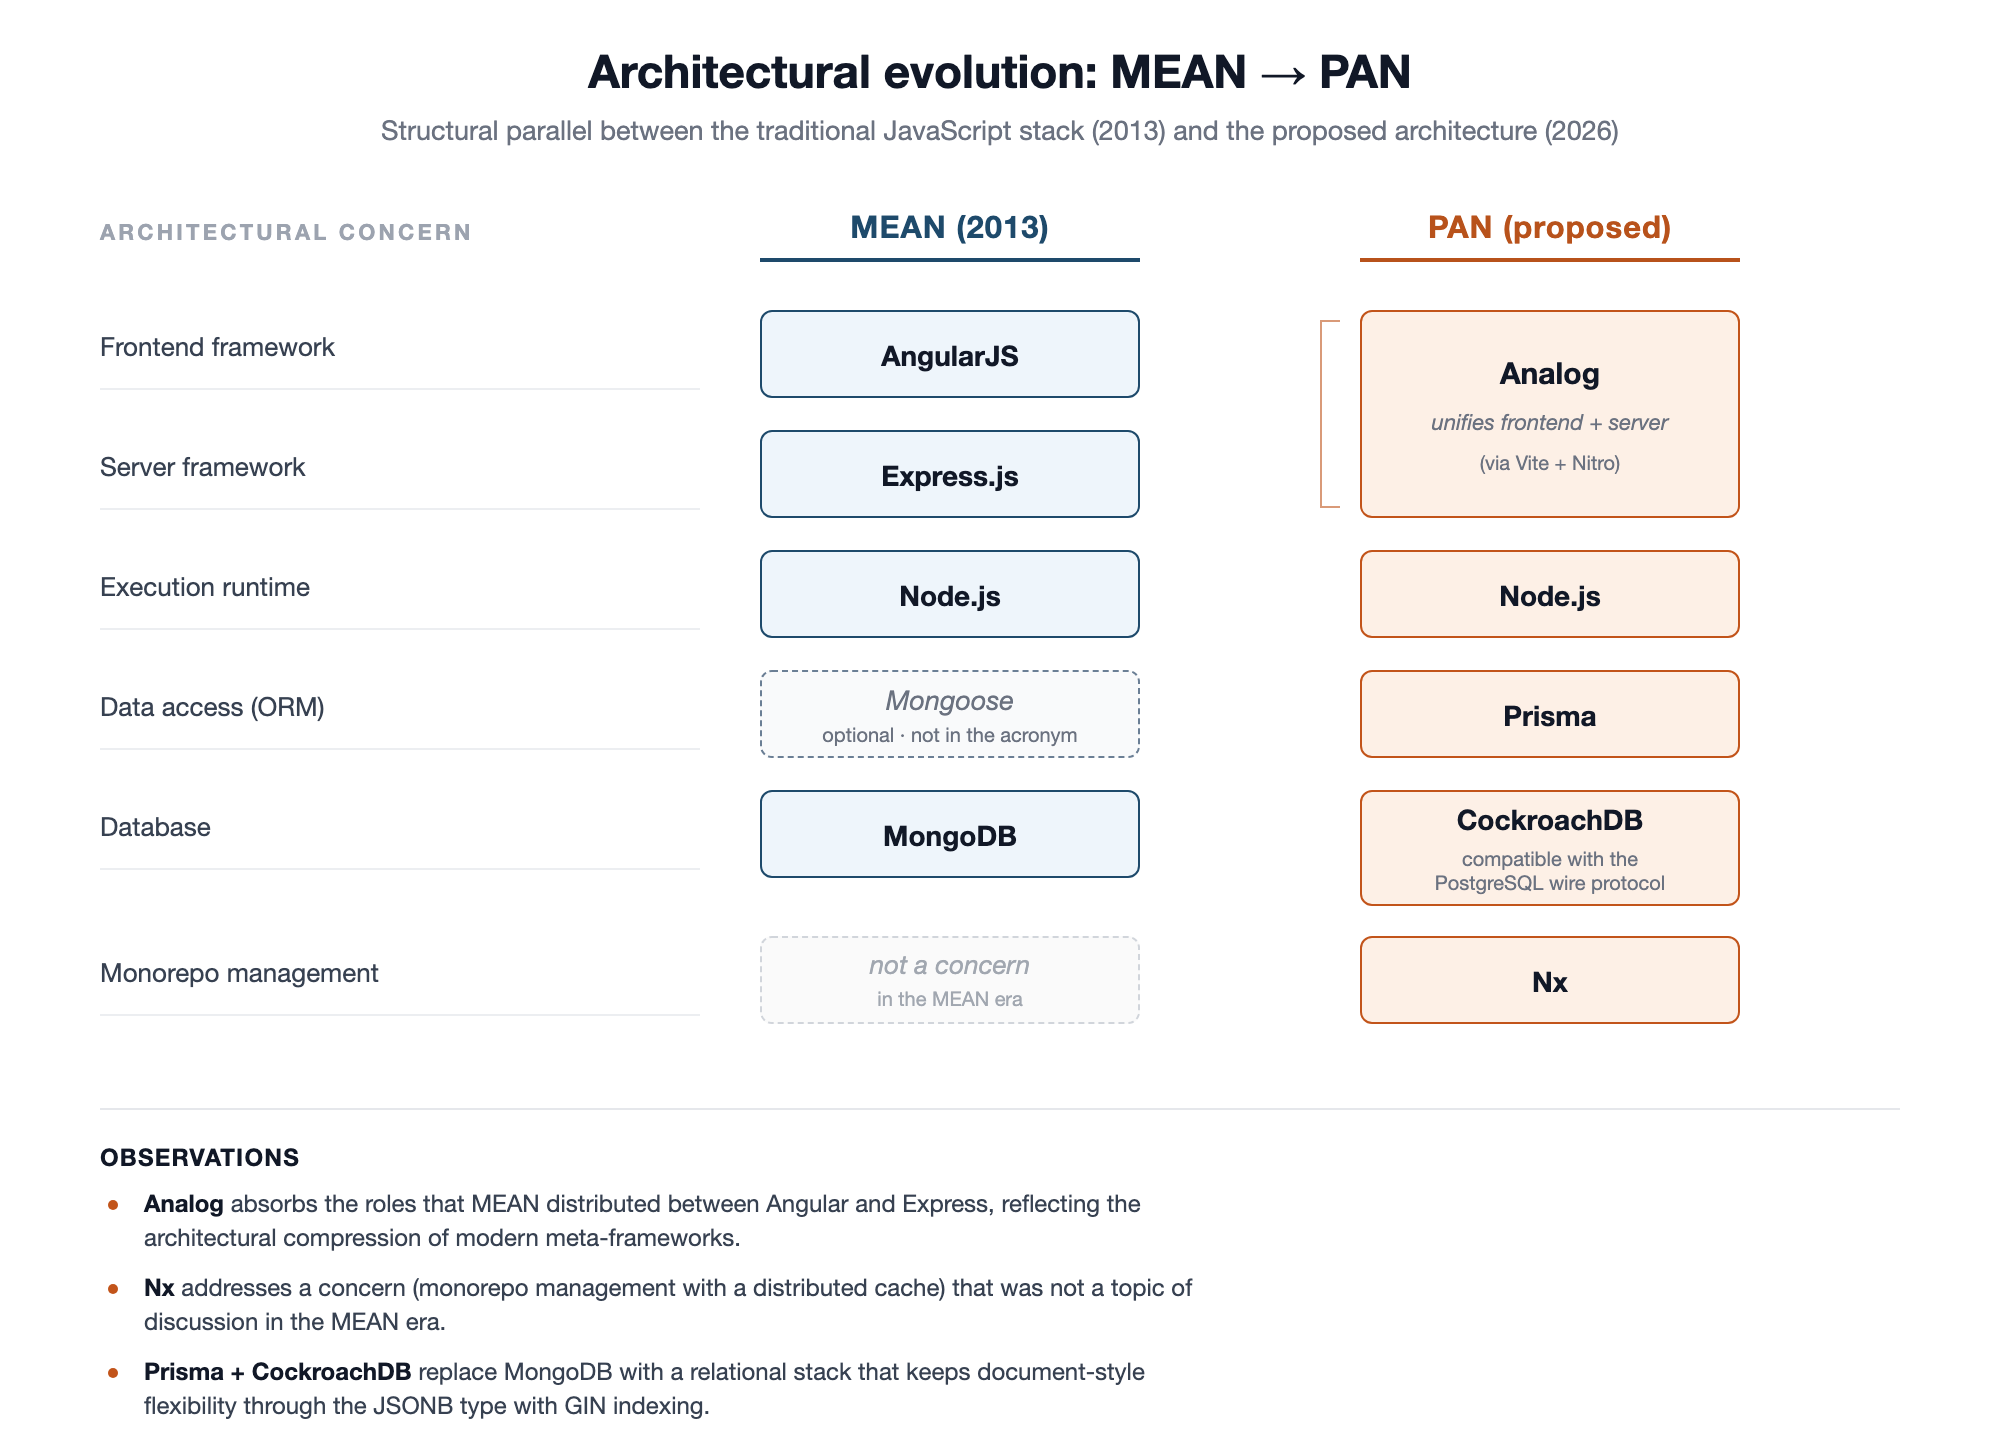
\includegraphics[width=1.11\textwidth]{mean-vs-pan-en}}
  \caption{Structural parallel between the \gls{mean} architecture (Karpov, 2013) and the \gls{pan} architecture proposed in this thesis. The diagram highlights the maturing of the ecosystem: \gls{analog} absorbs the roles distributed in \gls{mean} between \textit{Express} and \gls{angular}, and \gls{nx} addresses the concern of \gls{monorepo} organization which, in the \gls{mean} era, was not yet a topic of architectural discussion.}
  \label{fig:mean-vs-pan}
\end{figure}

\begin{table}[htbp]
\centering
\caption{Comparison between \gls{mean} (2013), the modern React stack and the \gls{pan} architecture.}
\label{tab:pan-vs-altele}
\small
\begin{tabularx}{\textwidth}{lYYY}
\toprule
\textbf{Aspect} & \textbf{\gls{mean} (2013)} & \textbf{MERN + \gls{nextjs} + Turborepo} & \textbf{\gls{pan}} \\
\midrule
Frontend         & \gls{angular} (legacy)  & React                  & \gls{angular} 21 \\
Meta-framework   & --- (Express)           & \gls{nextjs}           & \gls{analog} \\
Server runtime   & Node.js + Express       & Node.js + \gls{nextjs} & \gls{nitro} \\
API              & Manual REST             & API routes + optional \gls{trpc} & Mandatory \gls{trpc} \\
Shared types     & No                      & Partial (App Router)   & Automatic end-to-end \\
Database         & MongoDB                 & MongoDB or \gls{postgresql} & \gls{cockroachdb} \\
\gls{orm}        & Mongoose                & \gls{prisma} or Drizzle & \gls{prisma} \\
Monorepo         & ---                     & Turborepo              & \gls{nx} \\
Language         & JavaScript              & Partial \gls{typescript} & Pure \gls{typescript} \\
\bottomrule
\end{tabularx}
\end{table}

The major differences between \gls{pan} and the modern React stack are:

\begin{itemize}
  \item \textbf{Community.} \gls{pan} is built on \gls{angular}, a framework with a smaller usage share than React (\(50.1\,\%\) versus \(81.1\,\%\), \textit{State of JavaScript 2024}~\cite{stateOfJS2024}). This difference is both a practical limitation (fewer available developers, fewer \textit{third-party} \acrshort{ui} libraries) and an invitation to discipline --- \gls{angular} imposes a more structured organization by default, through dependency injection and strictly typed \textit{standalone} components.

  \item \textbf{Maturity.} \gls{nextjs} has almost a decade of evolution and extensive production adoption; \gls{analog} is under three years old and has a small community. \gls{pan} compensates by choosing \gls{angular} and \gls{nitro} (both mature individually) as base platforms, but accepts the community risk of \gls{analog}.

  \item \textbf{End-to-end typing.} In \gls{pan}, \gls{trpc} is a mandatory component of the architecture, not an optional one. This decision makes \gls{pan} more restrictive than the modern React stack (where you can choose REST, GraphQL or \gls{trpc} ad hoc), but eliminates the class of contract desynchronization errors between client and server.
\end{itemize}

\subsection{Technological framework}\label{sec:cadrul-tehnologic}

\subsubsection{Modern web architectures}\label{subsec:arhitecturi-web}

For a cooking application in which the user's first impression depends on HTML populated from the very first visit, the client-side rendering (\acrshort{csr}) model of a classic \gls{angular} single-page application (\acrshort{spa}) was not enough.
The requirements of fast display, \acrshort{seo} for public recipes and subsequent on-page interactivity led to an architecture that splits the \gls{randare} work between the server and the client~\cite{analog,nitro}.

The \gls{randare} strategies relevant to the project are:
\begin{itemize}
  \item \textbf{\acrshort{csr}} (client-side rendering) --- used in \textit{\gls{kookio}} for the authenticated screens (planner, pantry), where interactivity comes first;
  \item \textbf{\acrshort{ssr}} (server-side rendering) --- for public pages with dynamic content (recipe feed, profiles), where the initial HTML must be complete;
  \item \textbf{\acrshort{ssg}} (static site generation) --- prerendering, at \textit{build} time, the pages whose content is completely stable; it is supported by \gls{analog}, but not used in the current version of the application, in which static pages are server-rendered as well;
  \item \textbf{hybrid architectures} --- combining these strategies on different routes, depending on the nature of the content~\cite{analog}.
\end{itemize}

I chose a hybrid full-stack architecture in which the frontend and the backend run in the same \gls{typescript} code base.
The decision is motivated practically: the types and validation schemas (\gls{trpc} with validation through \gls{zod} schemas) are shared at module level, and a single build step delivers both layers~\cite{trpc,zod}.

\subsubsection{Angular and server-side rendering}\label{subsec:angular-ssr}

I chose \gls{angular} as the frontend framework because its ecosystem natively provides the pieces I needed for \textit{\gls{kookio}}: strict typing, \textit{standalone} components, \gls{angular} Signals (reactive signals) and the \gls{angular} Material/CDK component set, consistent with respect to accessibility~\cite{angular_signals,angular_material}.

\acrshort{ssr} support in \textit{\gls{kookio}} comes from \textbf{\gls{analog}}, a \gls{metaframework} that extends \gls{angular} with:
\begin{itemize}
  \item \acrfull{ssr} and \acrfull{ssg} configurable per route,
  \item routing based on the file structure,
  \item integration of the server logic (\gls{nitro}, \gls{trpc}) in the same project~\cite{analog,analog_routing,nitro}.
\end{itemize}

For a public recipe page, \acrshort{ssr} makes the difference between a minimal HTML document until \gls{hydration} and HTML that is populated from the very first request --- important both for the user and for the \acrshort{seo} indexing on which the organic distribution of the content relies~\cite{analog}.

\subsubsection{Monorepo and orchestration with Nx}\label{subsec:monorepo-nx}

I organized \textit{\gls{kookio}} as a \gls{monorepo} using \textbf{\gls{nx}}: a single application (\texttt{apps/web}) and a set of libraries segmented by responsibility (\texttt{feature}, \texttt{prisma}, \texttt{server}, \texttt{shared})~\cite{nx}.

The libraries are grouped by role:
\begin{itemize}
  \item \texttt{feature/} --- user flows (\texttt{auth}, \texttt{shell}),
  \item \texttt{prisma-client} --- the schema, the generated client, the \gls{zod} schemas,
  \item \texttt{server/} --- the \gls{trpc} context, logging, middleware, server runtime utility functions,
  \item \texttt{shared/} --- \acrshort{ui}, utilities, simulated (\textit{mock}) data.
\end{itemize}

On top of this structure, \gls{nx} provides two essential mechanisms used systematically in the project: \texttt{nx affected} runs only the tasks (\texttt{lint}, \texttt{test}, \texttt{build}) touched by the current changes, and the \texttt{enforce-module-boundaries} rule rejects in \acrshort{ci} the imports that violate the library topology~\cite{nx}.

\subsubsection{tRPC and type sharing}\label{subsec:trpc}

Client--server communication in \textit{\gls{kookio}} uses \textbf{\gls{trpc}} (\textit{TypeScript Remote Procedure Call} --- typed remote procedure calls for \gls{typescript}): the procedures are declared once, in \gls{typescript}, on the server, and the \gls{angular} client invokes them directly, without an additional layer of API definitions~\cite{trpc}.

The concrete advantages I observed:
\begin{itemize}
  \item full \gls{typescript} inference eliminates the hand-written \glspl{dto} that appear in classic REST architectures,
  \item input validation is done through \gls{zod} schemas generated automatically from the \gls{prisma} schema~\cite{zod,prisma_zod_generator},
  \item refactorings that rename fields propagate instantly across both layers.
\end{itemize}

For \textit{\gls{kookio}}, in practice, this translated into the almost complete elimination of type checks at the client--server boundary: the contract is the compiler.

The limits of pure static typing also motivate the runtime validation layer. The taxonomy of undetectable bugs in~\cite{gao2017type} ranks string-content errors (\textit{StringError} --- malformed URLs, malformed queries) second by frequency, since the \texttt{string} type is opaque to most static type systems. Validation through \gls{zod} schemas at the \gls{trpc} boundary covers precisely part of this gap, checking at runtime formats, enums and constraints that the \gls{typescript} compiler cannot express.

\subsubsection{Persistence: Prisma and CockroachDB}\label{subsec:persistenta}

For persistence I chose \textbf{\gls{cockroachdb}} as the database and \textbf{\gls{prisma}} as the \gls{orm}~\cite{prisma_orm,cockroachdb}.
\gls{cockroachdb} is compatible with the \gls{postgresql} wire protocol, which means that the SQL tooling ecosystem (drivers, \texttt{psql} clients, \gls{prisma}) works without adaptations, while additionally offering native horizontal scaling capabilities.
Standard \gls{postgresql} focuses on vertical replication, whereas \gls{cockroachdb} adds native horizontal scaling on top of the protocol~\cite{cockroachdb}.

In the project, \gls{prisma} covers three responsibilities: declaring the schema in \texttt{schema.prisma}, generating a \gls{typescript} client with exact types for each model, and managing the versioned migrations applied at \texttt{deploy}~\cite{prisma_orm}.

To generate the \gls{zod} schemas I use \texttt{prisma-zod-generator}, which exposes a validatable copy of each model --- the source of truth is the \gls{prisma} schema, and the API and \acrshort{ui} layers consume derivatives of it~\cite{prisma_zod_generator}.

\subsubsection{Automated testing: Vitest and Playwright}\label{subsec:testare}

The test suite of \textit{\gls{kookio}} has two distinct layers: unit tests with \textbf{\gls{vitest}} for isolated logic and \acrlong{e2e} (\acrshort{e2e}) with \textbf{\gls{playwright}} for complete scenarios through a real browser~\cite{vitest,playwright}.

I chose \gls{vitest} because it already runs on \gls{vite} (the same bundler as the main application), which means there are no duplicated configurations or divergences between \texttt{nx test} and \texttt{nx build}~\cite{vitest,vite}.

\gls{playwright} covers the critical flows: authentication, completing \textit{onboarding}, adding to the pantry, viewing the planner.
The suite runs in \acrshort{ci} on every \acrshort{pr} targeting \texttt{test} before promotion to \texttt{main}~\cite{playwright}.

\subsubsection{Configuration and environment management}\label{subsec:configuratie}

Environment variables (Firebase keys, \gls{redis} URLs, \gls{vercel} secrets) are defined only once in the \gls{vercel} dashboard, separately per environment (\texttt{development}, \texttt{preview}, \texttt{production})~\cite{vercel_cli}.
This centralization eliminates \texttt{.env} files accidentally added to the Git history and keeps all branches in sync.

Locally, synchronization is done with \texttt{vercel env pull}, which writes a \texttt{.env.local} (excluded from version control through \texttt{.gitignore}) with the values of the current environment --- no secret is versioned in Git~\cite{vercel_cli}.
% 2-preliminaries.tex ends here

% 3-implementation.tex starts here
\section{Implementation}\label{cap:implementare}

\subsection{Implementation overview}

The previous chapter established the technology choices that make up the \textbf{\gls{pan}} architecture (defined in \secref{subsec:pan-definitie}). In what follows I describe how this pattern translates into the actual structure of the repository: a single \gls{analog} application under \texttt{apps/}, a set of \gls{nx} libraries grouped by responsibility under \texttt{libs/}, and a unified execution chain through which a request travels from the \gls{analog} server-side runtime to the \gls{trpc} and \gls{prisma} layers.

% Keep the heading + the ~14cm file tree together: if less than 15cm is left on
% the current page, start them on the next one rather than splitting the tree.
\needspace{15cm}
\subsubsection{Structure of the Nx monorepo}\label{subsec:structura-monorepo}
\vspace{0.3cm}
\begin{TreeVerb}
kookio/
├── apps/
│   ├── web/                    # Analog application (Angular 21 + SSR),
│   │                             runs both in the browser and as
│   │                             a server runtime (Nitro)
│   └── web-e2e/                # Playwright suite for the critical
│                                 flows (login, onboarding, pantry,
│                                 planner)
├── libs/
│   ├── feature/                # user-facing flows
│   │   ├── auth/               #   login, registration, session
│   │   ├── onboarding/         #   profile setup steps
│   │   ├── pantry/             #   pantry management
│   │   ├── plan/               #   daily planner
│   │   ├── recipes/            #   recipe feed and details
│   │   ├── groceries/          #   derived shopping list
│   │   ├── saved/              #   saved collections
│   │   ├── dashboard/          #   main authenticated screen
│   │   └── shell/              #   layout, topbar, navigation
│   ├── prisma-client           # Prisma schema, migrations,
│   │                             generated Zod schemas, derived types
│   ├── server/                 # auth, logger, trpc
│   │                             (server runtime helpers)
│   └── shared/                 # ui, utility, mock
│                                 (components, helpers, fixtures)
├── nx.json                     # global Nx configuration
├── package.json                # main project manifest
├── tsconfig.base.json          # TypeScript config + path aliases
├── vercel.json                 # Vercel routes, headers and build
└── vitest.workspace.ts         # Vitest workspace (all projects)
\end{TreeVerb}
\vspace{0.3cm}

In practice, a change in \texttt{libs/feature/pantry} triggers only the checks for the affected library and for the modules that depend directly on it (via \texttt{nx affected}), not for the entire repository \cite{nx}. The topology between groups (\texttt{feature/} does not import from \texttt{feature/}, \texttt{shared/} depends on nothing internal) is enforced automatically by the \texttt{enforce-module-boundaries} rule, checked in \acrshort{ci}.

\subsubsection{End-to-end application flow}\label{subsec:flux-capcoada}

At a high level, a request goes through three layers: \textit{\Gls{analog} (\acrshort{ui} and \acrshort{ssr})} \(\rightarrow\) \textit{\acrshort{trpc} (typed API)} \(\rightarrow\) \textit{\gls{prisma} (data access)} \cite{analog,trpc,prisma_orm}. The transitions between layers do not go through an additional layer of manual serialization --- the \gls{typescript} types are shared from end to end, and input validation at the \gls{trpc} boundary uses \gls{zod} schemas derived from the \gls{prisma} schema \cite{trpc,zod,prisma_zod_generator}. The step-by-step breakdown of a concrete request (from the initial \acrshort{ssr} to the subsequent calls from the browser) can be found in \secref{subsec:flux-executie}, and the corresponding sequence diagram in \figref{fig:flux-executie}. The overall picture of the components and of the externally managed services is shown in \figref{fig:arhitectura}.

\begin{figure}[htbp]
  \centering
  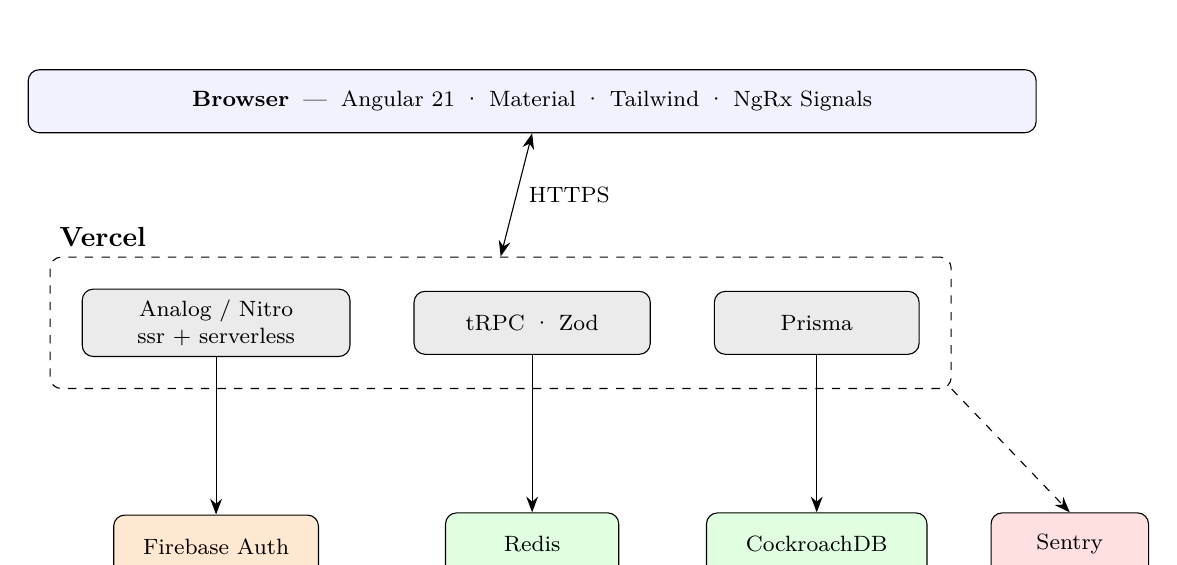
\begin{tikzpicture}[
    font=\footnotesize,
    >={Stealth[length=2mm]},
    L/.style={draw, rounded corners, align=center, minimum height=8mm, inner sep=4pt},
  ]
    \node[L, fill=blue!5, minimum width=128mm] (client)
      {\textbf{Browser} \;---\; Angular 21 · Material · Tailwind · NgRx Signals};

    \node[L, fill=black!8, minimum width=30mm, below=20mm of client] (trpc) {tRPC · Zod};
    \node[L, fill=black!8, minimum width=34mm, left=8mm of trpc] (analog) {Analog / Nitro\\\acrshort{ssr} + serverless};
    \node[L, fill=black!8, minimum width=26mm, right=8mm of trpc] (prisma) {Prisma};
    \begin{scope}[on background layer]
      \node[draw, dashed, rounded corners, fit=(analog)(trpc)(prisma), inner sep=4mm] (vercel) {};
    \end{scope}
    \node[anchor=south west, font=\bfseries] at (vercel.north west) {Vercel};

    \node[L, fill=orange!18, minimum width=26mm, below=20mm of analog] (fb) {Firebase Auth};
    \node[L, fill=green!12, minimum width=22mm, below=20mm of trpc] (redis) {Redis};
    \node[L, fill=green!12, minimum width=28mm, below=20mm of prisma] (db) {CockroachDB};
    \node[L, fill=red!12, minimum width=20mm, right=8mm of db] (sentry) {Sentry};

    \draw[<->] (client.south) -- node[right=1pt]{HTTPS} (vercel.north);
    \draw[->] (analog.south) -- (fb.north);
    \draw[->] (trpc.south) -- (redis.north);
    \draw[->] (prisma.south) -- (db.north);
    \draw[->, dashed] (vercel.south east) -- (sentry.north);
  \end{tikzpicture}
  \caption[Overall architecture of the application]{Overall architecture:
    the browser (\gls{angular}) communicates over HTTPS with the \gls{vercel}
    platform, which hosts the \gls{analog}/\gls{nitro} runtime (\acrshort{ssr} +
    serverless functions), the \gls{trpc} layer (with \gls{zod} validation) and
    the \gls{prisma} client. Persistence and cross-cutting services are managed
    externally: \gls{cockroachdb} (data), \gls{redis} (cache,
    \textit{rate-limiting}), Firebase (authentication) and \gls{sentry} (error
    monitoring).}
  \label{fig:arhitectura}
\end{figure}

\subsection{Implementation of the application}

Whereas the previous section justified the technology choices, this one shows how each choice looks in the repository: which files materialize it, which conventions apply it and what concrete constraints it imposed at the code level. For each technology, the emphasis is no longer on \textit{why} it was chosen, but on \textit{what it actually produced} once integrated into \textit{\gls{kookio}}.

\subsubsection{Modern web architectures}\label{subsec:arhitecturi-implementare}

The \gls{randare} configuration of \textit{\gls{kookio}} is concentrated in \texttt{apps/web/vite.config.ts}: the \texttt{analog} plugin is called with \texttt{ssr: true}, with no prerendered routes. Thus, \acrshort{ssr} is the rendering mode for all the application's routes, including pages with stable content such as \texttt{/about}; \acrshort{ssg}, although supported by \gls{analog}, is not used, so that every response goes uniformly through the server runtime \cite{analog}.

On the \acrshort{ssr} path, the distinction between public routes (\texttt{/recipes}, \texttt{/legal/\allowbreak attributions}) and authenticated ones (\texttt{/pantry}, \texttt{/plan}) does not show up in the \gls{randare} strategy, but in what the server executes before serving the page: authenticated routes go through a \textit{guard} (route interceptor) that issues a redirect to \texttt{/login} if the Firebase session is missing, visible to \gls{playwright} as \texttt{ERR\_ABORTED} on Chromium and handled through \texttt{waitUntil: 'commit'} in the \acrshort{e2e} tests.

\subsubsection{Library topology and the absence of a repository layer}\label{subsec:topologie-biblioteci}

The application's \textit{feature} libraries are vertical slices: each one represents a complete user flow (\texttt{auth}, \texttt{onboarding}, \texttt{pantry}, \texttt{plan}, \texttt{recipes}) and contains the components, the state stores (NgRx Signals \textit{stores}) and the services that flow depends on. The topology enforced by the \gls{nx} \texttt{enforce-module-boundaries} rule is acyclic: \texttt{apps/} \(\rightarrow\) \texttt{libs/feature/} \(\rightarrow\) \texttt{libs/server/}, \texttt{libs/shared/}, \texttt{libs/prisma-client}, and \texttt{libs/feature/X} cannot import from \texttt{libs/feature/Y}. Communication between features happens through \texttt{providedIn: 'root'} state stores or through the \gls{trpc} procedures exposed by \texttt{libs/server/trpc} \cite{nx,nx_boundaries,trpc}. The project's dependency graph, collapsed onto the four \textit{scope} domains, is shown in \figref{fig:nx-graph}.

\begin{figure}[htbp]
  \centering
  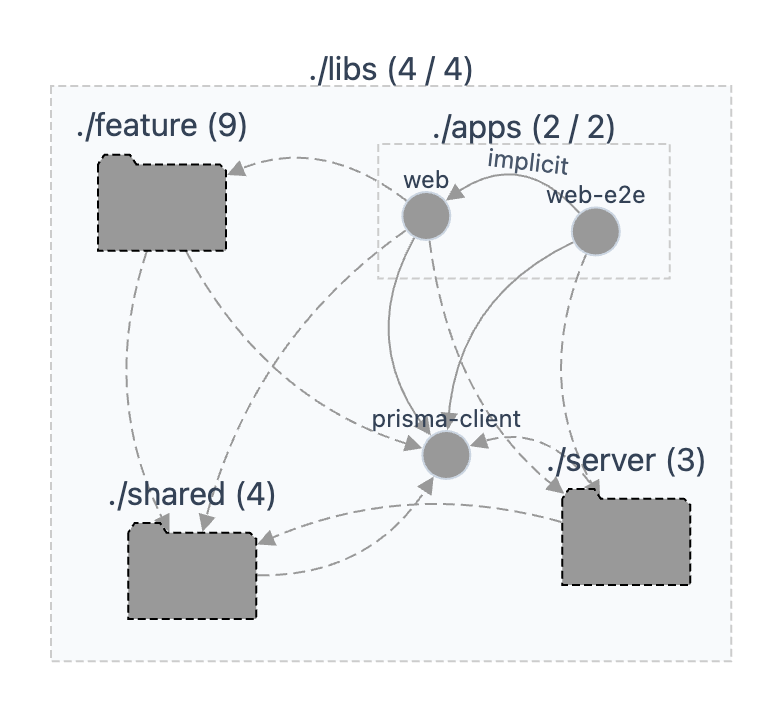
\includegraphics[width=0.7\textwidth]{graph-all}
  \caption[The project's \gls{nx} dependency graph]{The project's dependency
    graph (\gls{nx}), collapsed onto the four \textit{scope} domains:
    \texttt{feature} (9 libraries), \texttt{server} (3), \texttt{shared} (4) and
    \texttt{prisma-client}, plus the \texttt{web} and \texttt{web-e2e}
    applications. The arrows show the dependency relationship; the topology is
    acyclic (\texttt{apps} \(\rightarrow\) \texttt{feature} \(\rightarrow\)
    \texttt{server}, \texttt{shared}, \texttt{prisma-client}), with the lower
    layers having no dependencies on the upper ones.}
  \label{fig:nx-graph}
\end{figure}

Organizing the feature libraries as vertical slices (each a complete user flow --- \texttt{auth}, \texttt{pantry}, \texttt{plan}), rather than as horizontal layers matching the processing stages, reflects Parnas's central conclusion: it is almost always incorrect to begin the decomposition of a system on the basis of a flowchart \cite{parnas1972}. Parnas contrasts the two modularizations of the KWIC system --- one by stages (input \(\rightarrow\) circular shift \(\rightarrow\) alphabetizing \(\rightarrow\) output), the other by information hiding --- and shows that in the first a change such as the storage format propagates into every module, whereas in the second it stays confined to a single one. Because design decisions transcend the time order of execution, modules do not correspond to processing steps. In \gls{pan}, this observation translates into the structural prohibition \texttt{feature/X} \(\not\rightarrow\) \texttt{feature/Y}: slices communicate through \gls{trpc} procedures or root-level state stores, not horizontally through stages.

The acyclic topology enforced by the \gls{nx} \texttt{enforce-module-boundaries} rule also corresponds to the \gls{uses} relation that Parnas requires to be a loop-free partial ordering \cite{parnas1972}. The benefits he attributes to this ordering can be found in \textit{\gls{kookio}}: the lower layers (\texttt{shared}, \texttt{server}, \texttt{prisma}) can be used without the upper ones, and “cutting off” the upper features leaves a reusable trunk --- exactly the property that allows a new feature library to be added incrementally without touching the rest of the application. It is important, however, to mark the distinction Parnas makes explicitly: a hierarchical structure (an acyclic \gls{uses} relation) and a “clean” decomposition (through information hiding) are two desirable but independent properties. The \gls{nx} \texttt{enforce-module-boundaries} rule guarantees the former --- the dependency graph stays acyclic ---, but does not by itself guarantee that each library actually hides a changeable design decision. The latter remains a discipline applied when drawing the boundaries: the \acrshort{ci} rule prevents the topology from degrading, not the absence of a real secret in a poorly delimited library.

The backend and frontend code coexist in the same repository: the \gls{prisma} client and the generated \gls{zod} schemas live in \texttt{libs/prisma-client}, and their types are imported directly into the \gls{angular} components \cite{prisma_zod_generator}. There is no classic object-oriented \textit{repository} layer between the \gls{trpc} procedures and \gls{prisma}; the routers call \texttt{ctx.prisma} directly, and the multi-step transactions --- including writes that touch several domains, such as the atomic transfer of bought items from the shopping list into the pantry (\texttt{groceries.addBoughtToPantry}, \secref{subsec:lista-cumparaturi}) --- use \texttt{prisma.\$transaction} \cite{trpc,prisma_transactions}. This direct coupling does not reduce the testability of the procedures: the \gls{trpc} context remains an injection point through which \texttt{ctx.prisma} can be replaced with a test double, a mechanism detailed in \secref{subsec:testare-validare}.

\subsubsection{Angular and server-side rendering}\label{subsec:angular-ssr-implementare}

The application's routes are defined based on the file structure (\textit{filesystem-based}) under \texttt{apps/\allowbreak web/\allowbreak src/\allowbreak app/\allowbreak pages/}: a file \texttt{about.page.ts} exposes \texttt{/about}, \texttt{cook.\allowbreak [recipeId].\allowbreak page.ts} exposes a dynamic route with a parameter, and a co-located \texttt{cook.\allowbreak [recipeId].\allowbreak server.ts} loads data before \gls{angular} renders the component \cite{analog,analog_routing}. Each \texttt{*.page.ts} is a \textit{default export} and is loaded on demand (\textit{lazy loading}) by the \gls{analog} router; there is no centralized routes file.

The application-level \acrshort{ssr} configuration is minimal: \texttt{app.config.ts} registers file-based routing, the HTTP client and hydration with replay of the events captured in the interval between \acrshort{ssr} and \gls{hydration} (the concrete mechanism is described in \secref{subsec:flux-executie}) \cite{analog}. Each import added to \texttt{app.config.ts}, however, carries a cost amplified by \acrshort{ssr}: the module is evaluated on the critical path of every route, and aggregating \textit{barrel} files (re-exports of the \texttt{export *} kind) are not eliminated by \gls{vite} in the development environment. The practical constraint is to import directly, through sub-paths, only the tokens actually used, leaving heavy components (Material datepicker, autocomplete) to be loaded from the level of the page that uses them.

\subsubsection{Data management with Prisma and CockroachDB}\label{subsec:gestionarea-datelor}

The database schema lives at \texttt{libs/prisma-client/schema.prisma}, alongside the migrations managed by \gls{prisma} and the \texttt{prisma-zod-generator} generator, which produces a validatable copy of each model in \gls{zod} form \cite{prisma_orm,prisma_zod_generator}. The complete schema --- the 20 models and the relationships between them --- is shown as an entity-relationship diagram in \anxref{anexa:model-date}. The derived types (initial data sets, form inputs, payloads for \gls{trpc} routes) are built by composition --- \texttt{.pick()}, \texttt{.omit()}, \texttt{.extend()} --- directly on top of the generated schemas, so that renaming a field in \texttt{schema.prisma} propagates automatically to the consumers \cite{prisma_zod_generator}.

Two structural decisions support this arrangement. First, the public \texttt{@kookio/prisma-client} entry point is safe to run in the browser: it exports only types and \gls{zod} schemas, while the \texttt{PrismaClient} instance is isolated under the \texttt{@kookio/prisma-client/server} sub-path, whose import is blocked by ESLint in frontend code \cite{prisma_orm}. Second, the \gls{prisma} instance is extended with an automatic \textit{retry-on-conflict} for the \gls{cockroachdb}-specific \textit{serializable} error codes (\texttt{P2034}, \texttt{P2036}, \texttt{40001} and the \textit{restart transaction} message); all write operations (\texttt{create}, \texttt{update}, \texttt{upsert}, \texttt{delete} and the \texttt{*Many} variants) go through this \textit{wrapper}, and the multi-step transactions are designed to be idempotent so that they can be retried automatically \cite{prisma_transactions,cockroachdb}.

The concrete connection to \gls{cockroachdb} is made through the \textit{driver adapter} pattern introduced in \gls{prisma} 7: the \texttt{PrismaClient} instance receives at construction an explicit adapter (\texttt{@prisma/adapter-pg}) that encapsulates the \texttt{pg} connection \textit{pool} for the \gls{postgresql} wire protocol \cite{prisma_orm,cockroachdb}. The connection pool is sized for the \textit{serverless} execution model: at most five connections per instance, with a connection \textit{timeout} of 10 seconds and a query \textit{timeout} (\texttt{statement\_timeout}) of 20 seconds, so that an ephemeral instance does not exhaust the database's connection quota and a stuck query does not hold a connection indefinitely. Starting with this version, \gls{prisma} drops the native engine written in Rust: the client runs entirely in JavaScript, and the database URL is moved from \texttt{schema.prisma} into a dedicated \texttt{prisma.config.ts} file. This separation between the typed client (generated from the schema) and the actual transport driver makes it possible, in principle, to change the data source without regenerating the client --- a flexibility that is useful for integration testing against a local database and for future migrations between \gls{postgresql}-compatible providers.

Compound uniqueness constraints are declared in \texttt{schema.prisma} and enforced at the database level --- for example \texttt{@@unique([userId, date, slotType])} on \texttt{MealSlot}, or the \texttt{userId}--\texttt{ingredientCatalogId} pair on \texttt{PantryItem} ---, and \gls{prisma} automatically generates the \textit{compound key} forms (of the kind \texttt{where: \{ userId\_ingredientCatalogId: \{ \ldots \} \}}) for the corresponding lookup queries \cite{prisma_orm}.

\subsubsection{Building the initial data set}\label{subsec:pipeline-date}

The data the database is populated with --- the catalog of ingredients, categories, culinary areas and the 594 recipes --- is not written by hand, but derived from a public source, \textit{TheMealDB}, through an offline fetching and cleaning pipeline. The source, however, is a \textit{crowd-sourced} database: the instructions are free text, the measures appear in heterogeneous forms (\texttt{"2 tbsp heaped"}, \texttt{"1/2 cup"}), and the ingredient names contain duplicates, plural forms and typos. Cleaning this data into a form that conforms to the \gls{prisma} schema requires deterministic, versioned and reproducible transformations --- which is why the pipeline is built as a set of \gls{typescript} scripts separate from the application, under \texttt{research/the-meal-db/}, each one consuming the artifact of the previous phase and producing a JSON \textit{snapshot}.

The pipeline runs in five phases. The \textit{fetching} phases query the source API --- the catalog (categories, areas, ingredients) and the recipes, the latter discovered by scanning the 26 letters of the alphabet, with up to 20 ingredient positions parsed for each recipe from the source's flat structure. The \textit{catalog cleaning} phase normalizes the names to a stable \texttt{snake\_case} key (diacritics removed, whitespace collapsed) used as a unique identifier throughout the pipeline, and auto-classifies each ingredient into one of the categories through an ordered list of twelve matching rules (\textit{first-match-wins}, with \texttt{PRODUCE} as the final catch-all rule; ingredients that do not match remain unclassified, for manual review). The \textit{recipe cleaning and enrichment} phase derives the structured fields (described below), and a final \textit{residual fixes} phase applies, directly to the canonical files, a set of idempotent mechanical rewrites.

One structural decision of the pipeline deserves highlighting: the separation between the automatic output and the canonical source. The cleaning scripts never overwrite the \texttt{recipes.json} file committed to the repository --- they write to an intermediate snapshot (\texttt{clean-recipes.json}), and promotion into the canonical source happens through a deliberate manual review step. As a result, hand-made refinements (re-segmentations of steps that the automatic parser missed, transcription fixes) survive re-running the pipeline, while purely mechanical fixes remain automated and idempotent. The source of truth is versioned, not regenerated on every run.

Three of the enrichment transformations are heuristics with an algorithmic role, not mere reformatting. Estimating the \textit{number of servings} maps each ingredient to its mass in grams --- volumes through the density of water, piece-type units through a table of per-piece weights --- excluding pure flavoring ingredients (salt, oil, vinegar) and negligible units; the total bulk mass is divided by a tunable constant of \(400\) g per serving --- an indicative weight for a main-course serving, chosen pragmatically and tunable, with no claim to nutritional value --- and clamped to the interval \([1, 12]\), with a default of \(2\) servings for recipes with fewer than two bulk ingredients or under \(200\) g of usable data. \textit{Difficulty} is a three-tier \textit{bucket} (\texttt{EASY}, \texttt{MEDIUM}, \texttt{HARD}) derived from a complexity score of \texttt{ingredients} \(+\ 2 \times\) \texttt{steps} --- steps weighted double, since they reflect effort, not just the shopping list --- relative to the median of the scores across the entire catalog: below \texttt{median} \(\times\ 0.8335\) is \texttt{EASY}, above \texttt{median} \(\times\ 1.1665\) is \texttt{HARD}, the rest \texttt{MEDIUM} (the bands are the median \(\pm\ 1/6\), so they yield an even split only for a uniform distribution; since recipe complexity is right-skewed, there are more \texttt{EASY} than \texttt{HARD} recipes). Finally, \textit{measure parsing} turns the free-text strings into \texttt{(quantity, \texttt{MeasureUnit}, notes)} triples --- ranges take the lower bound, and unrecognized units are moved into the notes field, without losing information.

The residual fixes phase is where the reality of crowd-sourced data shows most clearly: twenty-four distinct transformations, each idempotent (run a second time, it changes nothing). Rather than an enumeration, they fall into four classes of data quality issues: \textit{typographic and Unicode normalization} (typographic apostrophes and curly quotes brought to ASCII, Unicode fractions parsed, zero-width characters removed); \textit{referential integrity} (rewriting ingredient names from plural to singular according to the merge plan, so that recipes link correctly to the catalog, plus deduplicating ingredients repeated within the same recipe, which the \texttt{@@unique([recipeId, ingredientCatalogId])} constraint would reject); \textit{reconstruction of the step structure} (splitting steps that contained internally numbered sub-steps, removing header steps and metadata leaked as instructions); and \textit{regeneration of derived fields} (\textit{kebab-case} slugs from the title, with explicit mapping of extended Latin characters, and reclassifying difficulty after the step restructuring shifted the global median). Idempotence is guaranteed structurally --- each transformation matches only the uncorrected form or stops when the current state equals the target --- so the pipeline can be safely re-run after any manual refinement.

\subsubsection{Client–server communication with tRPC}\label{subsec:comunicare-trpc}

The \gls{trpc} routers are defined under \texttt{libs/server/trpc/src/lib/routers/}, one router per domain (\texttt{auth}, \texttt{pantry}, \texttt{onboarding}, \texttt{meal-plan}, \texttt{recipes}, \texttt{cooking-session} and others). Each procedure is composed from one of three \textit{builders}: \texttt{publicProcedure} (an alias for \texttt{procedure}, exposed anonymously, without authentication, defined in \texttt{libs/server/trpc/src/lib/trpc.ts}), \texttt{protectedProcedure} (requires a Firebase session verified in \texttt{createContext}) and \texttt{onboardedProcedure} (additionally requires \texttt{onboardingDone === true} on the user, otherwise it rejects the request with \texttt{PRECONDITION\_FAILED}), the last two declared in \texttt{libs/\allowbreak server/\allowbreak trpc/\allowbreak src/\allowbreak lib/\allowbreak middlewares/\allowbreak auth.ts} \cite{trpc,trpc_middleware}. The convention is a structural one: a \texttt{grep} for the builder used in a router immediately shows what surface the endpoint exposes, without having to inspect each locally composed \textit{middleware} layer.

On the client side, the \gls{trpc} instance is created in \texttt{apps/web/src/trpc-client.ts}: the Firebase \textit{ID token} is attached as the HTTP \texttt{Authorization} header through the \texttt{headers} option of the transport \textit{link} (a reactive \textit{signal} read on every request), and a dedicated \texttt{authAwareFetch} (i) proactively refreshes the token when it expires in less than five minutes, (ii) retries the request once with a new token on a \texttt{401} response, (iii) resolves relative URLs to absolute form in the \acrshort{ssr} context (Node.js has no implicit base for \texttt{fetch('/api/\ldots')}). In this configuration the \gls{trpc} procedures return RxJS \texttt{Observable}s, and the \gls{angular} consumers choose between \texttt{from(\ldots).pipe(\ldots)} for a reactive stream and \texttt{await firstValueFrom(from(\ldots))} for a single result \cite{trpc}.

\subsubsection{Auxiliary h3 routes and the Redis infrastructure}\label{subsec:rute-h3-redis}

Besides the \gls{trpc} handler (\texttt{apps/\allowbreak web/\allowbreak src/\allowbreak server/\allowbreak routes/\allowbreak api/\allowbreak trpc/\allowbreak [trpc].ts}), the application exposes two additional \texttt{h3} routes: \texttt{/api/health} for the \textit{healthcheck} and \texttt{/api/internal/bench-db} for the \gls{cockroachdb} latency benchmark (used in the evaluation section). A single \texttt{h3} \textit{middleware} (\texttt{apps/web/src/server/\allowbreak middleware/security.ts}) covers two cross-cutting requirements: an explicit \texttt{404} for static files that are not found (\texttt{/assets/*}, \texttt{/fonts/*} and others) --- to avoid the situation in which \acrshort{ssr} would return \texttt{200} with HTML for a \textit{bundle} replaced between deploys --- and rejecting with \texttt{404} the usual automated scanning patterns (\texttt{/wp-admin}, \texttt{.env}, \texttt{.git}, \texttt{.php} extensions). Security headers are applied at two levels. At the network \textit{edge}, through \texttt{vercel.json}, \gls{hsts} is applied with a one-year duration and \texttt{includeSubDomains}, which forces HTTPS access across the entire domain. The \gls{csp} policy is issued per request by a dedicated \gls{nitro} plugin (\texttt{apps/\allowbreak web/\allowbreak src/\allowbreak server/\allowbreak plugins/\allowbreak csp.ts}): for each HTML response, the plugin generates a unique \textit{nonce}, attaches it to the application's inline scripts and includes it in the header, keeping \texttt{script-src} strict (the own origin plus the nonce) without allowing the execution of arbitrary inline code; the remaining sources stay limited to the own origin, with a \textit{frame} exception for the Firebase authentication domain.

The Redis component lives in \texttt{apps/web/src/server/infra/} and is designed to tolerate unavailability. \texttt{getRedis()} is a singleton with a 60-second \textit{circuit breaker}: after a failed connection, the following calls \textit{fail fast} instead of recreating the client \cite{redis}. On the read path (\texttt{groceries.list}), a utility function silently catches Redis failures and returns the empty set, so that the page renders without the “bought” state; on the write path, the response includes a \texttt{persisted: false} field if Redis is unavailable, allowing the client to keep the \textit{optimistic update} and display a notification. Rate limiting (\textit{rate-limiting}, \texttt{rateLimitFixedWindow}) uses an \texttt{INCR + EXPIRE} fixed window and is applied both to the \textit{benchmark} route (10 requests per window) and to the \gls{trpc} handler: 10 requests for registration (\texttt{auth.register}) and 300 for the other procedures. In line with the unavailability-tolerance principle described above, rate limiting is \textit{fail-open} --- if Redis does not respond, the request is let through instead of being rejected, so that a failure of the \textit{cache} layer does not block authentication or writes. Also to protect the free-tier Redis instance, a weekly scheduled task (\textit{cron}) calls the \texttt{/api/cron/\allowbreak redis-keepalive} route, keeping it active to prevent the auto-suspension cycle.

\subsubsection{Logging and observability}\label{subsec:jurnalizare}

The \gls{logging} layer is isolated in \texttt{libs/server/logger/}: a single \gls{pino} instance is created with an environment-dependent transport --- \texttt{pino-pretty} with \textit{colorize} and a short timestamp in development, raw JSON in production (\gls{vercel}) \cite{pino}. On the production path, the instance applies an explicit list of redacted fields (\textit{redact list}: \texttt{password}, \texttt{*.token}, \texttt{authorization}) to prevent credentials from leaking into the logs.

Besides the global logging instance, \texttt{createLogger(namespace, bindings)} returns a child \textit{logger} with a \textit{namespace} label from a fixed set (\texttt{audit}, \texttt{http}, \texttt{trpc}, \texttt{prisma}) plus additional \textit{bindings} --- for example \texttt{createLogger('trpc', \{ router: 'pantry' \})} produces \texttt{ns: 'trpc'} alongside \texttt{router: 'pantry'} on every emitted entry ---, and \texttt{createAudit(bindings)} returns a logger specialized for audit events (with the \texttt{audit: true} flag applied automatically). Messages are always structured --- \texttt{logger.info(\{ userId, action \}, 'message')} --- not string interpolations, so that the resulting logs can be filtered directly on the aggregation platform.

On top of the logging layer, error monitoring in production is provided by \gls{sentry}, integrated symmetrically on the client and the server and inactive (\textit{no-op}) until an ingestion key (\acrshort{dsn}) is configured, so that development environments and deployments prior to the configuration remain untouched. On the client, a global \texttt{ErrorHandler} captures unhandled errors, and a \texttt{reportError} \textit{helper} isolated in \texttt{libs/shared/observability/} is called at the error-handling points in the \textit{stores} --- the \texttt{catchError} blocks that consume the error to turn it into interface state ---, making otherwise silent failures visible as well. On the server, the \texttt{wrap()} function in \texttt{libs/server/logger/} becomes the single capture point: the \texttt{error} and \texttt{fatal} methods forward the \texttt{err} field to \texttt{Sentry.captureException} before delegating to \gls{pino}, so that every \texttt{log.error(\{ err \})} call in the \gls{trpc} routers reports automatically, without instrumenting each error point. The \texttt{@sentry/node} client is initialized only once, at server startup, through a \gls{nitro} \textit{plugin} that also registers a \textit{hook} for unhandled errors, filtered to \texttt{5xx} codes so as not to report \texttt{4xx} client errors. The symmetry is deliberate: unhandled errors are caught by the global \textit{handlers} on both ends, and handled ones by the two single capture points --- \texttt{reportError} on the client, \texttt{wrap()} on the server. Besides errors, the client also collects performance transactions through a \textit{tracing} integration with a sampling rate of 10\,\%, enough to observe the pages' vital metrics without exceeding the free-tier quota. At build time, the \texttt{@sentry/\allowbreak vite-plugin} \textit{plugin} uploads the \textit{source maps} to \gls{sentry} and removes them from the delivered \textit{bundle}: generated in \textit{hidden} mode, without the \texttt{sourceMappingURL} comment, they are never served to the client, and each deployment is tagged with a \textit{release} equal to the Git \textit{commit} \textit{hash}, so that a production error points exactly to the \textit{deploy} that introduced it \cite{sentry}.

\subsubsection{Execution flow of a request}\label{subsec:flux-executie}

The flow summarized in \secref{subsec:flux-capcoada} unfolds in three stages.

\textbf{Stage~1 (initial rendering).} The HTTP request reaches the \gls{analog} server-side runtime (based on \gls{nitro}), and the \gls{angular} instance is executed on the server to produce the initial HTML \cite{analog,nitro}.

\textbf{Stage~2 (querying the persistence layer).} The \gls{angular} components trigger calls to the \gls{trpc} procedures of the server-side layer; each procedure validates its inputs with a \gls{zod} schema derived from the \gls{prisma} schema and uses \texttt{ctx.prisma} to query \gls{cockroachdb} \cite{trpc,zod,prisma_zod_generator,prisma_cockroachdb}. The results propagate back through the \gls{trpc} layer to the components that take part in the initial rendering.

\textbf{Stage~3 (hydration and subsequent interaction).} The rendered HTML reaches the browser, and the \gls{angular} instance takes over through \gls{hydration} --- the DOM tree produced on the server is reused, and the events captured in the meantime are replayed by \texttt{withEventReplay()} \cite{analog}. From then on, subsequent interactions call the \gls{trpc} procedures directly from the browser, without a new \gls{randare} on the server \cite{trpc}. \figref{fig:flux-executie} shows this flow as a sequence diagram.

\begin{figure}[htbp]
  \centering
  \resizebox{\textwidth}{!}{%
  \begin{sequencediagram}
    \newthread{br}{Browser}
    \newinst[2.5]{sv}{Analog / Nitro}
    \newinst[2.5]{tr}{tRPC}
    \newinst[2]{pr}{Prisma}
    \newinst[2]{db}{CockroachDB}

    \begin{call}{br}{HTTP GET /route}{sv}{initial HTML}
      \begin{call}{sv}{procedure (Zod validation)}{tr}{result (SuperJSON)}
        \begin{call}{tr}{ctx.prisma.<op>}{pr}{data}
          \begin{call}{pr}{SQL}{db}{rows}
          \end{call}
        \end{call}
      \end{call}
    \end{call}
    \postlevel
    \begin{call}{br}{direct tRPC call (post-hydration)}{tr}{response}
      \begin{call}{tr}{ctx.prisma.<op>}{pr}{data}
      \end{call}
    \end{call}
  \end{sequencediagram}}
  \caption[Sequence diagram of a request]{Sequence diagram of a
    request. \textbf{Initial rendering (\acrshort{ssr}):} the HTTP request reaches
    the \gls{analog}/\gls{nitro} runtime, which queries the persistence layer
    through the \gls{trpc} (with \gls{zod} validation) \(\rightarrow\) \gls{prisma}
    \(\rightarrow\) \gls{cockroachdb} layers and returns the initial HTML.
    \textbf{Subsequent interaction:} after hydration, calls go directly
    from the browser to \gls{trpc}, without a new server-side rendering.}
  \label{fig:flux-executie}
\end{figure}

\subsubsection{Testing and validation}\label{subsec:testare-validare}

The \gls{vitest} suite is orchestrated by \texttt{vitest.workspace.ts} at the root of the repository, which automatically collects all the \texttt{vite.config.*} and \texttt{vitest.config.*} files from the \gls{nx} projects \cite{vitest,vite}. The specification files (\textit{specs}, \texttt{*.spec.ts}) are co-located with the tested code, both in the \textit{feature} libraries and in the server libraries (for example \texttt{pantry.router.spec.ts} next to \texttt{pantry.router.ts}). Granularity is the guiding principle: \texttt{nx affected -t test} runs only the specs touched by the current changes.

At the level of the server libraries, the \gls{trpc} procedures are tested in isolation, without starting an HTTP server and without a real database: each spec builds a fake context in which \texttt{ctx.prisma} is a test double with \texttt{vi.fn()} methods declared exactly for the operations touched by the procedure, and the procedure is invoked through \texttt{appRouter.createCaller(ctx)} \cite{trpc,vitest}. Since the \gls{prisma} client reaches the procedures through the context, not through a direct import, the context takes over the isolation role that a \textit{repository} layer would have had: its absence (\secref{subsec:topologie-biblioteci}) does not sacrifice testability, it only moves the injection point into the context.

The \gls{playwright} suite lives at \texttt{apps/web-e2e/} and has its own \texttt{global-setup.ts} that warms up all the application's routes before the first \textit{worker} process starts --- a measure needed to avoid the time constraints at the first start of \gls{vite} in the development environment \cite{playwright}. The critical flows (authentication, registration, completing \textit{onboarding}, adding to the pantry, viewing the planner) go through the interface in Chromium; protected routes use \texttt{waitUntil: 'commit'} to avoid the \texttt{ERR\_ABORTED} error produced by \gls{angular} redirects during \gls{hydration}.

The discipline most visible in practice applies to refactorings that change the dependencies injected into a shared component: the tests of the library in question keep passing (the local \textit{stubs}, test stand-ins, are updated), but the specs of the dependent modules may fail with \texttt{NullInjectorError}. To detect these regressions, \texttt{nx affected -t test} is run, which follows the \gls{nx} dependency graph and runs everything that is affected \cite{nx}.

\subsubsection{Development and deployment}\label{subsec:dezvoltare-deploy}

Environment configuration is centralized in the \gls{vercel} dashboard, separately for \texttt{production}, \texttt{preview} and \texttt{development} \cite{vercel_cli}. Locally, \texttt{vercel env pull} synchronizes the values of the current environment into a \texttt{.env.local} (excluded from version control through \texttt{.gitignore}), removing the need for any secret to be versioned in Git.

Promotion between environments follows the \texttt{dev} \(\rightarrow\) \texttt{test} \(\rightarrow\) \texttt{main} flow. The \texttt{dev} branch feeds the development \textit{Preview} environment; the \texttt{test} branch triggers the \acrshort{e2e} suite on the testing \textit{Preview} environment before promotion to \texttt{main}, and the \texttt{main} branch feeds the production \textit{deploy} in the \texttt{fra1} region (Frankfurt) \cite{vercel_cli}.

The production build runs \texttt{nx build web} with \texttt{NODE\_OPTIONS=\allowbreak --max-old-space-size=6144}.
The default V8 heap limit is insufficient for bundling the entire \gls{angular} Material stack in the \gls{nitro} context: the phases that transform the abstract syntax tree (AST) and generate the \textit{source maps} accumulate large volumes of temporary objects, and the build fails with \texttt{JavaScript heap out of memory} before completing.
Raising the limit to 6\,GB provides the necessary headroom for both phases.
\gls{prismaclient} is regenerated in the automated \textit{pipeline} --- the \texttt{generate} target is a dependency of the \texttt{build} target ---, so that the \gls{typescript} client and the \gls{zod} schemas derived from \texttt{schema.prisma} are always in sync with the data model before the consumers are compiled \cite{prisma_orm}. Since \gls{prisma} 7 no longer ships a platform-dependent native engine (the client runs entirely in JavaScript through a \textit{driver adapter}), regeneration concerns only the typed code, not binaries specific to the execution environment.

\subsubsection{Architectural patterns discovered during implementation}\label{subsec:pan-patterns}

Besides the structural principles established \textit{a priori} (\secref{subsec:pan-definitie}), implementing the \textit{\gls{kookio}} application exposed three architectural patterns that were not predictable from the initial choices, but that consolidated into generalizable lessons for any \gls{pan} project. Unlike the intrinsic limitations of the stack (\secref{subsec:pan-limitari}), the patterns described here are reusable \textit{solutions}, codified in the project's guidelines repository to prevent the same problem from recurring:

\begin{itemize}
  \item \textbf{Authenticated SSR loaders require client-side hydration of authenticated data.} When first written, the \texttt{*.server.ts} loaders co-located with the dynamic routes called authenticated \acrshort{trpc} procedures directly through \texttt{appRouter.createCaller(ctx)}, assuming that the Firebase session from \texttt{createContext} is available both on the first \acrshort{ssr} and on subsequent client-side navigation. The assumption was false: on client-side navigation, \gls{analog} executes the \textit{loader} as an ordinary \texttt{fetch} that does not propagate the \texttt{Authorization} header with the Firebase \textit{ID token}, and the authenticated procedures respond with \texttt{401}. The correct pattern, codified in the repository: the \textit{loader} loads only public data (\textit{recipes.byId}, \textit{about page content}), while authenticated data (the availability of ingredients in the pantry, the “saved” state of a recipe, the user's preferences) is hydrated afterwards, from the browser, through the \gls{trpc} client with \texttt{authAwareFetch}. In terms of general applicability, the pattern comes down to the observation that \acrshort{ssr} and \textit{Bearer token} authentication do not coexist for free in any hybrid meta-framework --- any reader evaluating \gls{pan} for their own project should audit this dimension before relying on \acrshort{ssr} \textit{loaders} for sensitive data.

  \item \textbf{Route names in file-based routers must be semantic, not numeric.} When building the page for the \texttt{500} error code, the natural choice was a \texttt{/500} route (parallel to the already working \texttt{/404}). At runtime, the route did not activate: the server responded with \texttt{200} and the HTML of the home page. The cause, uncovered through gradual investigation, was a quirk of the \gls{analog} file-based router: \textit{all-numeric} segments are interpreted as invalid dynamic parameters, and the \textit{matcher} silently falls through the list of routes without signaling a configuration error. The correct pattern, codified in the repository: \textit{semantically} named routes (\texttt{/server-error}, \texttt{/not-found}, \texttt{/maintenance}) instead of numeric codes. In terms of general applicability, the pattern comes down to the observation that any file-based routing convention must separate \textit{numeric codes} (HTTP protocol artifacts) from \textit{route names} (semantic identifiers for the user) --- even if, in the world of protocols, the two seem interchangeable.

  \item \textbf{A single defensible heuristic for estimating quantities, two consumers.} The offline data cleaning pipeline (the \textit{seed} stage) and the runtime logic (pantry decrementing, shopping list derivation) initially consumed almost identical conversion heuristics, written separately --- a manual \texttt{INGREDIENT\_PIECE\_GRAMS} table at \textit{seed} time and their own \textit{carve-outs} at runtime ---, which forked every extension and, over time, produced behavioral divergences. Consolidating the two into a single source of truth (the pair of pure functions \texttt{toGrams}/\texttt{fromGrams} and the \texttt{IngredientCatalog.pieceGrams} column in the database schema) is detailed in \secref{subsec:algoritm-grame}. In terms of general applicability, the pattern comes down to a design rule: \textit{one defensible heuristic, two or more consumers, never one heuristic per consumer}. A critique of the estimate (for example, “the density of water is a poor approximation for oils”) applies to all consumers at once; an improvement propagates the same way.
\end{itemize}

The three patterns share a common structure: each emerged from \textit{implementation friction} (the \acrshort{ssr} \textit{loader} that responded with \texttt{401}, the \texttt{/500} route that did not activate, two almost identical heuristics written separately), and the solution was not adding functionality, but \textit{repositioning} the already existing piece at a level closer to the real invariant of the problem. From the standpoint of architectural auditing, this discovery pattern --- \textit{friction} \(\rightarrow\) \textit{lesson} \(\rightarrow\) \textit{codification} --- has been observed in the software engineering literature as a characteristic of evolutionary systems, in which the correct invariant is learned from implementation experience, not imposed by the initial design.

\subsection{Functional flows and product algorithms}\label{subsec:fluxuri-functionale}

The previous sections described how the architectural layer --- \gls{analog}, \acrshort{trpc}, \gls{prisma} --- materializes the \gls{pan} architecture at the code level. This section goes one level lower, to the \textit{product algorithms} that realize the application's value proposition: progressive filtering of recipes based on the pantry inventory, transactional decrementing of quantities after cooking, and automatic derivation of the shopping list from the planned slots. The three flows converge into a single \textit{estimation algorithm} that unifies the data cleaning pipeline (described in \secref{subsec:gestionarea-datelor}) with the production runtime logic.
Progressive filtering of recipes based on the pantry inventory (\secref{subsec:filtru-progresiv}) and automatic derivation of the shopping list (\secref{subsec:lista-cumparaturi}) operationalize two of the prevention strategies identified by Schanes et al.~\cite{schanes2018}: cooking with what is already stored at home and checking the inventory before shopping.

\subsubsection{Progressive recipe filtering}\label{subsec:filtru-progresiv}

On the \texttt{/recipes/match} route, the user sees the recipe catalog partitioned into three levels, labeled in the interface \textit{Alright} (all non-negligible ingredients are present in the pantry), \textit{Almost} (one to three non-negligible ingredients are missing) and \textit{All} (all public recipes, unfiltered). The \gls{trpc} procedure \texttt{recipes.match} receives a \texttt{level} field with exactly these three values (\texttt{'Alright'}, \texttt{'Almost'}, \texttt{'All'}), along with an optional \texttt{cursor} and a \texttt{limit} (default 20, maximum 50), and returns a page of recipes with the matching metadata the interface needs: the number of missing ingredients (\texttt{missingCount}), the names of the first three of them (\texttt{missingNames}) and the recipe's total number of ingredients (\texttt{totalIngredients}). The page also carries a \texttt{nextCursor} for pagination and a \texttt{partialScan} flag used by the client to automatically continue a scan interrupted by the examination budget.

The algorithm is, in essence, a \textit{set difference} between the recipe's ingredients and the contents of the user's pantry. For each recipe in the \texttt{PUBLIC} catalog, the procedure iterates through the list of \texttt{RecipeIngredient}s and skips the ingredients with a negligible unit (\texttt{TO\_TASTE}, \texttt{TO\_SERVE}, \texttt{GARNISH}, \texttt{PINCH}) --- salt, pepper, a parsley garnish and oil cannot block a recipe from the \textit{Alright} level just because they are missing from the explicit pantry records. The remaining ingredients are looked up in a map built from \texttt{pantryItem.findMany(\{ where: \{ userId \} \})}, compared at the level of \textit{existence} (the presence of the ingredient in the pantry, regardless of quantity). In the version delivered with this thesis, the quantity comparison is not performed; a rare false positive is preferred over unit logic that would duplicate the pipeline described in \secref{subsec:algoritm-grame}.

The decision to keep the matching logic simple --- \textit{presence}, not \textit{sufficient quantity} --- was taken deliberately: the cost of a false positive is low (a recipe appears as cookable although the user has an insufficient quantity of an ingredient), whereas the quantitative variant would duplicate the unit conversion logic of the grams pipeline (\secref{subsec:algoritm-grame}) at the matching boundary, with no proportional gain in perceived accuracy. For future development, the quantitative variant is built directly on top of that pipeline --- ingredients are normalized to grams before comparison, and the \textit{Alright} level requires the pantry to cover the recipe's consumption in grams for all non-negligible ingredients.

\subsubsection{The cooking session and transactional decrementing}\label{subsec:sesiune-gatit}

On the \texttt{/cook/:recipeId} route, the user goes through the recipe's steps and, at the end, a dialog offers a list of pre-filled quantities (proportional to the selected number of servings) for confirmation. On submission, the client calls \texttt{cookingSession.complete}, which decrements the pantry in a single \gls{prisma} transaction (\texttt{\$transaction}). For each confirmed \texttt{(ingredientCatalogId, consumedQuantity)}, the procedure looks up the corresponding row by the compound key \texttt{(userId, ingredientCatalogId)} (the \texttt{@@unique} constraint declared in \secref{subsec:gestionarea-datelor}), subtracts the consumed quantity from the existing quantity and --- this is where the estimation algorithm described in the next section comes in --- deletes the row if the remaining quantity drops below a minimum threshold (\texttt{0.5} g, the noise threshold of a pinch of salt). The entire operation runs atomically: either all the decrements go through and \texttt{cookingSession.completedAt} is updated, or nothing is applied.

Two implementation details are worth mentioning. First, the decrementing is done internally in grams (not in the display unit of the pantry row), to allow consumption in units different from the storage unit --- for example, a recipe calls for \texttt{200 g} of flour, but the user entered the flour as \texttt{0.5 kg}. The conversion back to the display unit happens at the end, before \texttt{prisma.update}. Second, if the user indicated a consumption greater than the quantity available in the pantry (an input mistake, or a recipe with a larger quantity entered later), the quantity is clamped to zero and the row is deleted, instead of receiving a negative value. These robustness behaviors at the edge of the data flow were validated through eighteen unit specification cases for \texttt{cookingSession.complete} at the time of the grams pipeline refactoring (28 May 2026).

\subsubsection{The grams pipeline: one heuristic, two consumers}\label{subsec:algoritm-grame}

The two previous flows --- progressive filtering (\secref{subsec:filtru-progresiv}) and the cooking session (\secref{subsec:sesiune-gatit}) --- depend on the same practical question: \textit{how do we convert quantities between heterogeneous units?} The recipe calls for \texttt{1 cup} of sugar and the pantry holds \texttt{500 g}; the recipe calls for \texttt{2 lemons}, but the pantry has only \texttt{1 piece}. A classic approach would separate each case (\textit{carve-out}): a converter for weights, a converter for volumes, a special rule for pieces. Over time, such layering produces branches that grow with every unit added.

The solution adopted in \textit{\gls{kookio}} is a pair of pure functions --- \texttt{toGrams} and \texttt{fromGrams} --- that normalize all quantities to grams before any operation and convert back to the display unit only at the end. The pipeline handles four classes of units --- weight, volume, pieces and taste/garnish ---, each with an explicit conversion rule; the per-class rules, the \texttt{allowDefault} option for pieces without a known weight and the implementation of the \texttt{toGrams} function are detailed in \secref{anexa:grams-detail}.

A single case is worth keeping here, since it is a design decision, not a mere conversion detail: the taste and garnish units (\texttt{TO\_TASTE}, \texttt{TO\_SERVE}, \texttt{GARNISH}) are treated as \texttt{0 g} and excluded from the shopping list. The \texttt{0 g} value is a consciously chosen modeling convention, not an unknown: it honors the intention of the recipe's author (the quantity is deliberately left “to taste”), avoids downstream noise (staple seasonings decremented on every cooking session or listed for shopping are not useful information in an application focused on the waste of bulk food) and keeps a neutral position with respect to dietary intake, which the application is not in a position to prescribe.

The \texttt{0 g} convention does, however, have a known limitation that follows directly from it: staple ingredients seasoned “to taste” (salt, oil, pepper) are not tracked at the quantity level, so their gradual depletion --- through small, repeated uses --- is not signaled to the user. The right solution to this gap is not assigning an arbitrary non-zero value (which would reintroduce the noise described above and would produce, in the absence of a warning infrastructure, data that nothing consumes), but a dedicated mechanism for tracking consumables, based on a state (\textit{in stock} / \textit{running low} / \textit{out of stock}) marked by the user, not on estimated mass. Such a module --- foreshadowed by the manual “running low” marker already present in the pantry interface --- is described as a direction for future development in \secref{sec:directii-viitoare}.

The structural decision this pipeline represents goes beyond the implementation detail: it is a \textit{unification} between two processes that previously used similar but separate heuristics. When generating the initial data sets (\textit{seeds}), an offline cleaning pipeline imported the \textit{TheMealDB} catalog and estimated the missing weights using a manual \texttt{INGREDIENT\_PIECE\_GRAMS} table built for this stage. At runtime, pantry decrementing (\secref{subsec:sesiune-gatit}) and shopping list derivation (\secref{subsec:lista-cumparaturi}) required the same conversions, but through separately written code. By extracting the \texttt{toGrams}/\texttt{fromGrams} functions into a common library (\texttt{libs/shared/utility}) and promoting the manual table to the \texttt{IngredientCatalog.pieceGrams} column, both processes now consume the same source of truth. From an auditing standpoint, a critique of the estimate (for example, “the density of water is a poor approximation for oils”) applies to both consumers at once; from an evolution standpoint, an improvement (a layer of per-category ingredient densities) propagates the same way. This design lesson is formulated as a generalizable architectural pattern in \secref{subsec:pan-patterns}.

The \texttt{toGrams}/\texttt{fromGrams} pair is a textbook application of information hiding \cite{parnas1972}: the changeable design decision --- the concrete way of converting between heterogeneous units (weight factors, approximating volumes through the density of water, the \texttt{pieceGrams} values for piece-type units) --- is isolated behind a stable interface, and the two consumers (the offline \textit{seed} pipeline and the runtime logic) depend exclusively on this interface, not on the implementation. The rule formulated above --- one defensible heuristic, two or more consumers --- restates the criterion according to which a module's interface should reveal as little as possible about its internal mechanism. The benefit is the one described by Parnas: a critique of the estimate (the density of water as a poor approximation for oils) or an improvement (a layer of per-category densities) applies to all consumers at once, because there is a single place where the decision is materialized.

\subsubsection{Deriving the shopping list}\label{subsec:lista-cumparaturi}

On the \texttt{/groceries} route, the shopping list appears as a \textit{set difference on ingredient identity} between the ingredients required by the planned slots and the contents of the pantry. The \texttt{groceries.list} procedure expands each slot with a recipe in the user's plan (all slots with a non-null \texttt{recipeId}) into the ingredients of the corresponding recipe, scales the quantities by the ratio \texttt{slot servings / recipe servings}, aggregates by \texttt{ingredientCatalogId} and completely removes any ingredient for which a row already exists in the pantry --- the removal comparison is made on \textit{presence}, not on quantity. Ingredients with a \textit{flavour-only} unit (\texttt{TO\_TASTE}, \texttt{TO\_SERVE}, \texttt{GARNISH}) are excluded from the list (salt, pepper and garnishes do not appear on the shopping list; \texttt{PINCH} is kept, having a non-zero mass (0.5 g)).

Reconciliation in grams does not happen when filtering the list, but when merging with the pantry: at the end, the \texttt{groceries.addBoughtToPantry} mutation transfers the items checked as “bought” directly into the pantry, merging them with any existing rows for the same ingredient. This merge uses the grams pipeline from \secref{subsec:algoritm-grame} --- it normalizes the quantities to grams, sums them and converts back to the storage unit of the existing row (or of the new item, if the row is missing). Piece-type items without a populated \texttt{pieceGrams} consume \texttt{DEFAULT\_PIECE\_GRAMS = 100} g through the \texttt{allowDefault} option, a \textit{graceful degradation} solution preferable to failing the operation because of a single incomplete ingredient.

The “bought” state of each item is persisted in \gls{redis} (\secref{subsec:rute-h3-redis}), allowing the user to continue the list on different \textit{devices} within the key's expiration window.

\subsection{Methodology and evaluation}\label{ch:evaluare}

\subsubsection{Experimental setup}\label{subsec:setare-experimentala}

All measurements were taken in the \gls{vercel} \textit{Preview} environment (the \texttt{fra1} region, Frankfurt), with \gls{cockroachdb} Serverless and \gls{redis} Cloud in the same region; the stack runs \gls{analog} on top of \gls{nitro}, with \acrshort{ssr} on the first request and \gls{hydration} on the client. The data set comes from deterministic test data sets (\textit{fixtures}, \texttt{libs/shared/mock/}) and from the initialization scripts (\textit{seed}, \texttt{libs/\allowbreak prisma-client/\allowbreak seed-data/\allowbreak catalog.json}, \texttt{recipes.json}).

All the measurement procedures are versioned in the project's repository: the benchmark route is defined in \texttt{apps/\allowbreak web/\allowbreak src/\allowbreak server/\allowbreak routes/\allowbreak api/\allowbreak internal/\allowbreak bench-db.get.ts}, the \acrshort{ci} flows are in \texttt{.github/workflows/}, and the configuration of the \acrshort{e2e} suite is in \texttt{apps/web-e2e/playwright.config.ts}. Each dimension is reproduced through a dedicated script in \texttt{scripts/}: persistence latency through \texttt{npm run bench:preview}, test coverage through \texttt{npm run bench:coverage}, and front-end performance --- the \gls{lighthouse} scores and the image payload --- through \texttt{npm run bench:lighthouse} and \texttt{npm run bench:images}, respectively; the scripts that query the \gls{vercel} environment require the corresponding access credentials.

\subsubsection{Indicators and procedures}\label{subsec:indicatori-proceduri}

\paragraph{Latency at the persistence layer.} The internal \texttt{/api/internal/bench-db} route executes, on each call, \(N=100\) successive read queries against \gls{cockroachdb} and \gls{redis}, respectively, reporting the arithmetic mean, the 50th percentile (\acrshort{p50}) and the 95th percentile (\acrshort{p95}). The cold/warm distinction operates at the level of the \textit{serverless} function invocation: the first call pays for the cold start of the instance and of the \textit{connection pool} to the database, while subsequent calls hit the already warmed-up instance. The cold call is reported separately from the median of the warm calls.

\paragraph{Reliability of the end-to-end (\acrshort{e2e}) tests.} The pass rate of the \gls{playwright} suite on Chromium, measured over the last ten runs on the \texttt{test} branch. WebKit also passes completely, and Firefox runs most of the tests, except a few authentication tests (marked \texttt{@no-firefox}), excluded because of a synchronization race at the level of the \textit{fetch} requests in the local development environment. In \acrshort{ci} only Chromium runs systematically; Firefox and WebKit are covered in manual runs before promotions to \texttt{main}.

\paragraph{Front-end performance.} \gls{lighthouse} is run on the home page of the application published at \texttt{kookio.app}, in the desktop and mobile profiles (the latter with network and CPU \textit{throttling}), reporting the median of several runs for the performance score and for the \gls{lcp}, \gls{cls} and \gls{tbt} metrics. Separately, the payload reduction of the image optimization is quantified: for each of the 594 images in the catalog, the original JPEG file is compared with the \gls{avif} variant delivered by the \gls{vercel} optimizer at the maximum configured width (\(w=960\)) --- a conservative bound, since smaller responsive widths save even more.

\paragraph{Unit test coverage.} Line coverage is reported over the entire source code of the libraries (\textit{all-source}: files not covered by any test are counted as \(0\,\%\), not omitted), aggregated from the per-project \gls{vitest} reports. The \texttt{web} application is excluded from this figure, because its test environment times out under coverage instrumentation; its user flows are validated by the \acrshort{e2e} suite.

\subsubsection{Results}\label{subsec:rezultate}

\begin{table}[htbp]
\centering
\caption{Summary of the results across the three measured dimensions.}
\label{tab:rezultate}
\begin{tabular}{lr}
\toprule
\textbf{Indicator} & \textbf{Value} \\
\midrule
\multicolumn{2}{l}{\textit{Latency at the persistence layer (\(N=100\) probes/call, median over warm calls)}} \\
\quad \gls{cockroachdb} (warm) --- mean & 1.79 ms \\
\quad \gls{cockroachdb} (warm) --- \acrshort{p50} & 1.71 ms \\
\quad \gls{cockroachdb} (warm) --- \acrshort{p95} & 2.07 ms \\
\quad \gls{cockroachdb} (\textit{cold start}) --- \acrshort{p50} / \acrshort{p95} & 2.6 / 6.4 ms \\
\quad \gls{redis} (warm) --- mean & 0.59 ms \\
\quad \gls{redis} (warm) --- \acrshort{p50} & 0.56 ms \\
\quad \gls{redis} (warm) --- \acrshort{p95} & 0.77 ms \\
\midrule
\multicolumn{2}{l}{\textit{Front-end performance (\gls{lighthouse}, median)}} \\
\quad Desktop score & 93 \\
\quad Mobile score (with \textit{throttling}) & 58 \\
\quad \acrshort{lcp} desktop / mobile & 1.5 / 8.3 s \\
\quad \acrshort{cls} (desktop / mobile) & 0.055 / 0 \\
\quad Image payload reduction (594 images, \(w=960\)) & \(-60.5\,\%\) \\
\midrule
\multicolumn{2}{l}{\textit{Coverage and testing}} \\
\quad Line coverage (library source code) & \(82.2\,\%\) \\
\quad Unit tests (\gls{vitest}) & 873 / 96 files \\
\quad \acrshort{e2e} tests (\gls{playwright}) & 14 / 7 flows \\
\quad \acrshort{e2e} pass rate on Chromium & \(100\,\%\) \\
\bottomrule
\end{tabular}
\end{table}

The results summarized in \tabref{tab:rezultate} confirm, within the limits explained in \secref{subsec:discutie-limitari}, the viability of the \gls{pan} architecture along the three evaluation axes: millisecond latencies at the persistence layer, solid front-end performance on desktop (score 93, zero \gls{cls}) with an acknowledged gap in the throttled mobile profile, a reduction of approximately \(60\,\%\) in the image payload across the entire catalog, a coverage of \(82.2\,\%\) of the library code and complete reliability of the critical end-to-end flows on the reference browser.

\subsubsection{Discussion and limitations}\label{subsec:discutie-limitari}

All measurements come from the \textit{Preview} environment, in the \texttt{fra1} region, without concurrent traffic --- so they do not capture the stack's behavior under load or in a multi-region setup. The \acrshort{e2e} suite runs only on Chromium in \acrshort{ci}, and the Firefox and WebKit test matrices are covered manually; automated promotion of the two would increase confidence in \textit{cross-browser} compatibility. In addition, both \gls{cockroachdb} and \gls{redis} run on the free tiers (with usage quotas and an \textit{auto-suspension} cycle for \gls{redis}) and are measured without concurrent traffic, which makes the reported latencies representative of a single-user regime, not of production at scale. Generalizing these results requires dedicated load tests and repeated measurements in a stable production environment. Moreover, these latencies are dominated by the free-tier managed providers --- the network time to the \texttt{fra1} region and the free-quota limitations ---, so they characterize the deployment infrastructure, not the \gls{pan} stack's own \textit{overhead}. Isolating this overhead would require a local, containerized benchmark (for example with Docker), without the network latency of the cloud providers --- a measurement direction left for future work.

Three limitations specific to the new measurements are worth pointing out. First, the persistence latencies vary noticeably between measurement sets --- the \acrshort{p50} median for \gls{cockroachdb} oscillated between approximately \(1.4\) and \(2.6\) ms ---, a consequence of the free tiers, the single region and the variable load; the value reported in \tabref{tab:rezultate} is the median of a set of warm calls, not a constant. Second, the \gls{lighthouse} score on the mobile profile reflects the aggressive \textit{throttling} applied by the tool (slow network and a four-times slower CPU), not the performance perceived on a real device --- the desktop profile remains in the good range. Finally, the \(82.2\,\%\) coverage concerns exclusively the library code, the \texttt{web} application being excluded for the reasons explained in \secref{subsec:indicatori-proceduri}.
% 3-implementation.tex ends here

% 4-conclusions.tex starts here
\section{Conclusions}\label{cap:concluzii}

I proposed the \textbf{\gls{pan}} architecture and validated it by implementing \textit{\gls{kookio}}, a full-stack \gls{web} application built entirely within the \gls{typescript} ecosystem on this model.
Starting from the preference for \gls{typescript} motivated in \capref{cap:preliminarii}, I translated this preference into a concrete stack: a single \gls{analog} application under \texttt{apps/web}, four groups of \gls{nx} libraries (\texttt{feature}, \texttt{prisma}, \texttt{server}, \texttt{shared}) with an acyclic topology enforced by \texttt{enforce-module-boundaries} in \acrshort{ci}, and an end-to-end \textit{\gls{analog}} \(\rightarrow\) \textit{\acrshort{trpc}} \(\rightarrow\) \textit{\gls{prisma}} flow described in \secref{subsec:flux-capcoada}.

Adopting the \textbf{\gls{pan}} architecture made it possible to eliminate the classic adaptation layers between frontend and backend.
The \acrshort{trpc} procedures call \texttt{ctx.prisma} directly, without a \textit{repository} layer (\secref{subsec:topologie-biblioteci}), and the \gls{zod} schemas consumed by \gls{angular} are derived from \texttt{schema.prisma} through \texttt{prisma-zod-generator} --- renaming a field propagates at compile time to all consumers.
The public \texttt{@kookio/prisma-client} entry point is safe to run in the browser (it exports only types and \gls{zod} schemas), while the \texttt{PrismaClient} instance is isolated under the \texttt{@kookio/prisma-client/server} sub-path, blocked by a dedicated ESLint rule in frontend code.

The combination of \textbf{\gls{angular}} and \textbf{\gls{analog}} delivered \acrshort{ssr} for all the application's routes, configured in a single place (\texttt{apps/web/vite.config.ts}).
The application-level \acrshort{ssr} configuration is minimal --- \texttt{provideFileRouter()}, \texttt{provideHttpClient(\ldots)} and \texttt{provideClientHydration(\allowbreak withEventReplay())} --- and the discipline identified in practice (\secref{subsec:angular-ssr-implementare}) is that every import added to \texttt{app.config.ts} carries an amplified cost on the critical path of every route, which is why the heavy Material components remain imported from the level of the page that uses them.

At the persistence layer, \textbf{\gls{prisma}} on top of \textbf{\gls{cockroachdb}} provided benefits directly observable at the code level.
Automatically generating the \gls{typescript} client and the \gls{zod} schemas from \texttt{schema.prisma} reduces the data contract to a single source of truth; the compound constraints declared as \texttt{@@unique} (\texttt{MealSlot} on \texttt{userId}--\texttt{date}--\texttt{slotType}, \texttt{PantryItem} on \texttt{userId}--\texttt{ingredientCatalogId}) are enforced at the database level, and the corresponding lookup queries use the automatically generated compound-key form.
To tolerate the retries that \gls{cockroachdb} may require under the default \textit{serializable} isolation, the \gls{prisma} instance is extended with an automatic \textit{retry-on-conflict} for the codes \texttt{P2034}, \texttt{P2036} and \texttt{40001} (plus the \textit{restart transaction} message); all write operations (\texttt{create}, \texttt{update}, \texttt{upsert}, \texttt{delete} and the \texttt{*Many} variants) go through this \textit{wrapper}, declared only once.

The testing process confirmed the value of combining two distinct levels.
The \textbf{\gls{vitest}} suite (orchestrated by \texttt{vitest.workspace.ts} at the root of the repository) covers isolated logic through specification files co-located with the tested code, and \texttt{nx affected -t test} runs only the specs touched by the current change.
The \textbf{\gls{playwright}} suite at \texttt{apps/web-e2e/} goes through the critical flows (authentication, \textit{onboarding}, pantry, planner) in Chromium and achieved a pass rate of \(100\,\%\) over the ten reference runs (\tabref{tab:rezultate}).
Two practices consolidated from the concrete \acrshort{ci} cycles: warming up the routes in \texttt{global-setup.ts} before the first \textit{worker} process starts, and \texttt{waitUntil: 'commit'} for protected routes, in response to the \texttt{ERR\_ABORTED} error produced by \gls{angular} redirects during hydration.

With respect to the objectives stated in \capref{cap:introducere}, I delivered a \acrlong{mvp} (\acrshort{mvp}) that covers the application's core flows: pantry management, daily meal planning, shopping list derivation and user \textit{onboarding}.
The \gls{monorepo} structure based on vertical slices (\texttt{libs/feature/auth}, \texttt{onboarding}, \texttt{pantry}, \texttt{plan}, \texttt{recipes}\ldots), in which \texttt{libs/feature/X} cannot import from \texttt{libs/feature/Y} --- a rule checked in \acrshort{ci} by \texttt{enforce-module-boundaries} --- allows extension with new flows as additional libraries, without structural changes to the existing application.

Overall, \textit{\gls{kookio}} shows that the \textbf{\gls{pan}} architecture can work coherently for a real full-stack \gls{web} application: the latencies measured on the \texttt{/api/internal/bench-db} route (median over warm calls of \(1.71\)~ms for \gls{cockroachdb} and \(0.56\)~ms for \gls{redis} --- \tabref{tab:rezultate}), the front-end performance (a \gls{lighthouse} score of 93 on desktop and a reduction of about \(60\,\%\) in the image payload across the entire catalog), the \(73.2\,\%\) coverage of the library code and the \(100\,\%\) pass rate of the \acrshort{e2e} suite on Chromium support this model within the limits explained in \secref{subsec:discutie-limitari} --- the \textit{Preview} environment, the single \texttt{fra1} region, free tiers for \gls{cockroachdb} and \gls{redis}, the \textit{cross-browser} test matrix covered manually and the absence of concurrent traffic, with the reported latencies reflecting a sequential regime, not performance at scale.

The main contribution of this thesis is the proposal and empirical validation of the \textbf{\gls{pan}} architecture as a coherent model for full-stack \gls{web} applications in the \gls{angular}/\gls{typescript} ecosystem, demonstrated through a working case study in the domain of reducing household food waste.

\subsection{Architectural decisions}\label{subsec:decizii-arhitecturale}

During the implementation, several initial decisions were refined, eliminated or reconfigured in response to implementation friction. The nine architectural decisions documented in the project's repository fall into three distinct categories, summarized in \tabref{tab:decizii-arhitecturale}: four \textit{simplifications} (eliminating systems that were built but had no real consumer), three \textit{unifications} (patterns discovered from friction and codified as rules, presented in detail in \secref{subsec:pan-patterns}) and two \textit{design decisions} (interface choices revised after implementation).

\begin{table}[htbp]
\centering
\caption{The nine documented architectural decisions, organized by category.}
\label{tab:decizii-arhitecturale}
\small
\begin{tabularx}{\textwidth}{lYY}
\toprule
\textbf{Category} & \textbf{Decision} & \textbf{Generalizable lesson} \\
\midrule
\multicolumn{3}{l}{\textit{Simplifications --- system built, zero real consumers, removal}} \\
\quad 1 & Removing biometric authentication (\textit{WebAuthn}) & The system was built in response to an anticipated, not an observed, requirement; no interface actually consumed it. \\
\quad 2 & Removing the role infrastructure (role-based access control) & The only consumer was a stub page for the administrator; the removal dropped the \texttt{Role} enum, the \texttt{User.role} column and the \texttt{roleProcedure} \textit{builder}. \\
\quad 3 & Flattening the \texttt{MealPlan} aggregate & The intermediate aggregate had no real consumer; the \acrshort{ui} worked directly with \texttt{MealSlot} on \texttt{(userId, date, slotType)}. The removal reduced the number of models in the schema by one. \\
\quad 4 & Removing the \texttt{core/} library group & The \textit{feature flags} subsystem and the configuration/security concerns were fully wired, but had no consumer (the router was not mounted, the \textit{guard} protected no route); the removal deleted the \texttt{core/config} and \texttt{core/security} libraries plus the \texttt{APP\_TRPC} token, and \texttt{core/logging} was absorbed into \texttt{server/logger} --- the taxonomy went from five to four groups. \\
\midrule
\multicolumn{3}{l}{\textit{Unifications --- implementation friction, codified lesson} (\secref{subsec:pan-patterns})} \\
\quad 5 & \acrshort{ssr} loaders require client-side hydration of authenticated data & The Firebase \textit{Bearer token} is not propagated through \texttt{fetch} on client-side navigation; loaders call only public procedures. \\
\quad 6 & Routes named semantically, not through numeric codes & The \gls{analog} file-based router silently falls through on \textit{all-numeric} segments; the solution: \texttt{/server-error} instead of \texttt{/500}. \\
\quad 7 & A single heuristic for estimating quantities, two consumers & The offline cleaning pipeline and the runtime logic now consume the same \texttt{toGrams}/\texttt{fromGrams} pair (\secref{subsec:algoritm-grame}). \\
\midrule
\multicolumn{3}{l}{\textit{Design decisions --- initial proposal, validated through later use}} \\
\quad 8 & \textit{Cook now} button moved from the \textit{FAB} \acrshort{ui} component to the topbar & The \textit{FAB} (\textit{floating action button}) component took up space without offering a visibility advantage over a button in the topbar. \\
\quad 9 & \textit{Quick actions} widget removed from the home page & The proposed quick actions were redundant with the bottom navigation bar plus the \textit{Cook now} button; the removal reduced the visual noise of the home page. \\
\bottomrule
\end{tabularx}
\end{table}

In the context of this bachelor's thesis, each decision represents an \textit{adjustment of the invariant} that the \gls{pan} architecture exposed when meeting a concrete use case. The simplifications (categories 1--4) show that a type-coherent stack makes it possible to quickly identify dead code by searching for \textit{consumer types}, not just import paths: if a \gls{trpc} procedure, a \textit{guard} or a \gls{prisma} model is not referenced anywhere in the frontend, removing it is safe at compile time. The unifications (categories 5--7) illustrate that the \gls{pan} architecture exposes friction that is not visible in the theoretical presentation of the stack (\secref{sec:cadrul-tehnologic}), but that arises from the interaction between components at runtime. The design decisions (categories 8--9) are independent of \gls{pan} as such, but show that the structural discipline of the stack does not prevent revising interface proposals --- the removed components were organized in their own libraries and could be taken out without touching the rest of the application.

The reflective tone of these decisions --- refined or removed when meeting a concrete case --- has a direct precedent in the founding article on information hiding: in the section “\textit{Improvement in Circular Shift Module}”, Parnas analyzes his own module and finds that its interface revealed more information than necessary (it imposed an ordering of the shifts), needlessly restricting the class of possible implementations --- an error he explicitly classifies as a design error \cite{parnas1972}. Documenting one's own revised decisions is therefore not a sign of project immaturity, but a practice present in the very text that introduced the principle.

\subsection{Limitations and trade-offs of the architecture}\label{subsec:pan-limitari}

Adopting \gls{pan} as an architecture is not without trade-offs.
This subsection lists them explicitly, so that a reader evaluating \gls{pan} for their own project can make an informed choice:

\begin{itemize}
  \item \textbf{The adoption curve.} \gls{pan} requires solid knowledge of \gls{angular} and of advanced \gls{typescript} (\textit{generics}, \textit{conditional types}, \textit{mapped types}). For a team without \gls{angular} experience, learning \gls{pan} costs significantly more than adopting a conventional \gls{nextjs}.

  \item \textbf{\gls{analog} maturity.} At the time of writing, \gls{analog} is a project with a community of a few thousand users and no major adoption in the corporate environment. The risk that certain production problems have no documented answer is real. The mitigation used in this thesis was selecting components that are mature individually (\gls{angular}, \gls{nitro}) and explicitly accepting the risk for the \gls{analog} orchestration layer.

  \item \textbf{Coupling to \gls{typescript}.} \gls{trpc} assumes that both ends of the communication are \gls{typescript}. \gls{pan} is not a viable option for applications that must expose a public API consumed by clients in other languages (Java, Go, Python). In such cases, GraphQL or OpenAPI remain more suitable choices.

  \item \textbf{Moderate vendor dependency.} Although \gls{pan} can be deployed on any Node.js-compatible infrastructure (\gls{nitro} supports \gls{vercel}, Netlify, AWS, Cloudflare, Bun, Deno), the integration with \gls{vercel} is the most well-trodden. Migrating to another provider is possible, but not effortless.

  \item \textbf{\gls{cockroachdb} at a small scale.} For applications under \(100{,}000\) requests per day, the operational complexity of \gls{cockroachdb} (the Raft consensus algorithm, the default \textit{serializable} isolation that requires retry logic) is disproportionate compared to standard \gls{postgresql}. \gls{pan} with classic \gls{postgresql} would be a simpler variant for applications that do not need real horizontal scaling.

  \item \textbf{Limited learning resources.} Community content (Stack Overflow, blog posts, courses) for \gls{pan} as such does not exist --- it exists only for the individual components. A developer facing a problem specific to the \gls{analog} \(+\) \gls{trpc} \(+\) \gls{prisma} \(+\) \gls{nx} integration has to build their own solution from first principles.

  \item \textbf{Gains given up by forgoing distribution.} The same review~\cite{soldani2018} identifies as major operational gains of microservices independent horizontal scalability (gain \#1, 31 studies), independent \textit{deployment} of components and the freedom to choose a distinct technology \textit{stack} for each service. \gls{pan} explicitly gives up the first two: the application is released as a single unit, and real scaling under concurrent traffic has not been characterized (\secref{subsec:discutie-limitari}). The third is the very negative of one of its founding principles --- end-to-end \gls{typescript} uniformity (\secref{subsec:pan-definitie}) is chosen precisely at the expense of per-component technological freedom. For a project that requires independent scaling of subsystems with divergent load profiles, or that must integrate services written in different languages, these trade-offs would tip the balance back towards a distributed architecture.
\end{itemize}

\gls{pan} is, therefore, not a universally applicable architecture.
It is an architecture for small teams with solid \gls{angular} knowledge building modern, monolithic (in the sense of single-unit release) and data-centric \gls{typescript} applications.
In this solution space, \gls{pan} offers a technological coherence and a structural discipline that React-based alternatives reach only through \textit{ad hoc} choices and conventions.

\subsection{Future directions}\label{sec:directii-viitoare}

The natural directions of evolution start from the limitations identified in \secref{subsec:discutie-limitari} and from the architectural trade-offs discussed in \secref{subsec:pan-limitari}.
At the infrastructure level, promoting \gls{cockroachdb} and \gls{redis} to paid tiers, together with enabling a second region beyond \texttt{fra1} (\gls{cockroachdb} natively supports cross-zone replication, which can be enabled without changes to the application code), would make it possible to characterize the stack under concurrent traffic.
In the area of testing, systematically including the Firefox and WebKit test matrices in \acrshort{ci} would strengthen confidence in \textit{cross-browser} compatibility beyond Chromium.
In terms of functionality, the existing \gls{redis} infrastructure (used for now to mark bought items on the shopping list and to rate-limit the benchmark route --- \secref{subsec:rute-h3-redis}) can be extended with an application-level \textit{caching} layer for public pages. Recommending recipes based on the pantry inventory is already covered by progressive filtering (\secref{subsec:filtru-progresiv}), and leveraging the preferences from \textit{onboarding} is partially implemented --- optional filtering by the preferred categories and culinary areas. Dietary restrictions are already collected and persisted in the \textit{onboarding} flow (a dedicated step writes them into \texttt{UserDietaryRestriction}), but they do not yet take part in the recommendation: what remains to be added is labeling the recipes with the restrictions they satisfy --- a \texttt{Recipe}--\texttt{DietaryRestriction} relationship currently absent from the schema, derivable from each recipe's ingredients --- after which the filter would plug into the same optional mechanism used for categories and areas.
Normalizing the ingredient catalog also contributes to matching accuracy: matching between recipe and pantry is done on the identity of the catalog ingredient, but some of the ingredients in the imported recipes use generic names (for example “flour” or “potatoes”) that have no direct counterpart in the catalog --- which contains only qualified variants, such as \textit{All purpose flour} or \textit{Plain Flour} --- so the recipes that call for them cannot reach the \textit{Alright} level starting from the pantry's contents. Extending the table of equivalences (\textit{aliases}) applied when importing the data (\secref{subsec:pipeline-date}) would reduce these mismatches and increase the proportion of fully covered recipes.
Along the same axis, a module for tracking consumables would address the limitation identified in \secref{subsec:algoritm-grame}: the staple ingredients seasoned “to taste” (salt, oil, pepper), which are currently not quantified, would be tracked at the level of a state (\textit{in stock} / \textit{running low} / \textit{out of stock}) marked by the user, and the items flagged as out of stock would automatically feed the shopping list, without resorting to mass estimates for quantities intentionally left to the cook's discretion.

Beyond the directions specific to the \textit{\gls{kookio}} product, the \gls{pan} architecture itself remains extensible along several axes not explored in the case study:

\begin{itemize}
  \item \textbf{Real-time communication.} \gls{trpc} supports \textit{subscriptions} over WebSocket or Server-Sent Events; a natural line of evolution is integration with a message broker (\gls{redis} Pub/Sub, NATS) for notifications to authenticated clients.

  \item \textbf{Functions at the network edge (\textit{edge functions}).} \gls{nitro} allows partial deployment at the \textit{edge} (\gls{vercel} Edge Functions, Cloudflare Workers). \gls{trpc} procedures that do not require \gls{prisma} can be moved to the \textit{edge} to reduce geographical latency.

  \item \textbf{Mobile applications.} The \gls{angular} stack supports native mobile applications through Capacitor or NativeScript; the \texttt{shared} and \texttt{prisma} libraries of a \gls{pan} project are directly reusable between a \gls{web} application and a mobile one.

  \item \textbf{Internationalization.} \gls{angular} i18n combined with multilingual \gls{analog} routing (routes parameterized by a language prefix) covers the case of multilingual applications without architectural changes.
\end{itemize}

The acyclic topology of the \gls{monorepo} allows these extensions to be made incrementally: a new library in \texttt{libs/feature/} with its own \gls{trpc} router is added without touching the rest of the application.
% 4-conclusions.tex ends here

\clearpage

\begin{appendices}
% 5-appendix-demo.tex starts here
% \raggedbottom for this appendix: the screenshot figures use [htbp] and the
% walkthrough paragraphs are short, so \flushbottom from the body would stretch
% inter-paragraph glue into gaps. Same rationale as the data-model appendix.
\raggedbottom


\section{Demonstration of the \textit{\gls{kookio}} application}\label{anexa:demo}

This appendix documents the main functional flow of the \textit{\gls{kookio}} application, as evidence that the \acrlong{mvp} (\acrshort{mvp}) described in \secref{cap:implementare} is operational from end to end. The screenshots capture a real user's journey --- from the pantry inventory, through meal planning and the shopping list, to the cooking session that decrements the stock. The final section relocates here the implementation detail of the unit conversion pipeline, kept in the body of the thesis only at the level of the design decision (\secref{subsec:algoritm-grame}).

\subsection{The main flow: from setup to cooking}\label{anexa:demo-flux}

The demonstrated journey covers the application's value chain, from the initial account setup to the automatic stock update after cooking: the user sets their preferences, declares what they have in the pantry, sees what they can cook, plans their meals, derives the shopping list for what is missing and, after cooking, the pantry is decremented.

\begin{figure}[htbp]
  \centering
  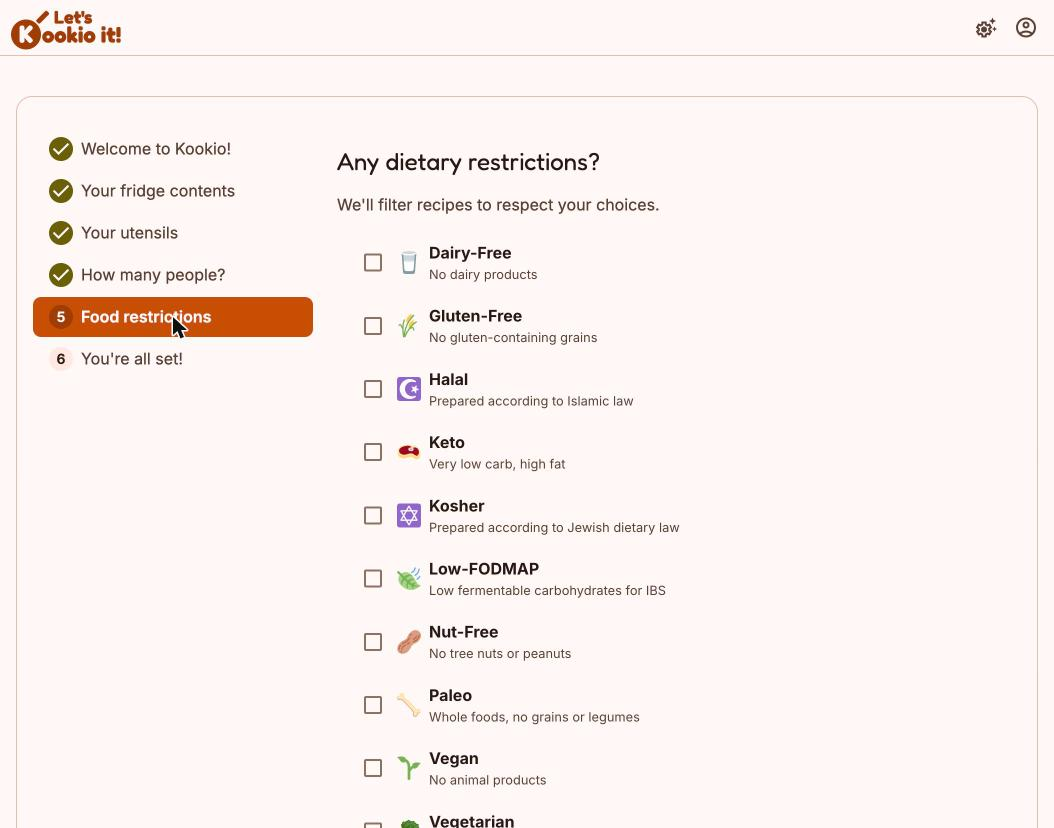
\includegraphics[width=0.66\textwidth]{kookio-demo-onboarding}
  \caption{Onboarding (\texttt{/onboarding}): the initial setup steps --- culinary preferences (categories and areas), dietary restrictions and available utensils --- persisted on completion and used later for filtering recipes.}
  \label{fig:demo-onboarding}
\end{figure}

\begin{figure}[htbp]
  \centering
  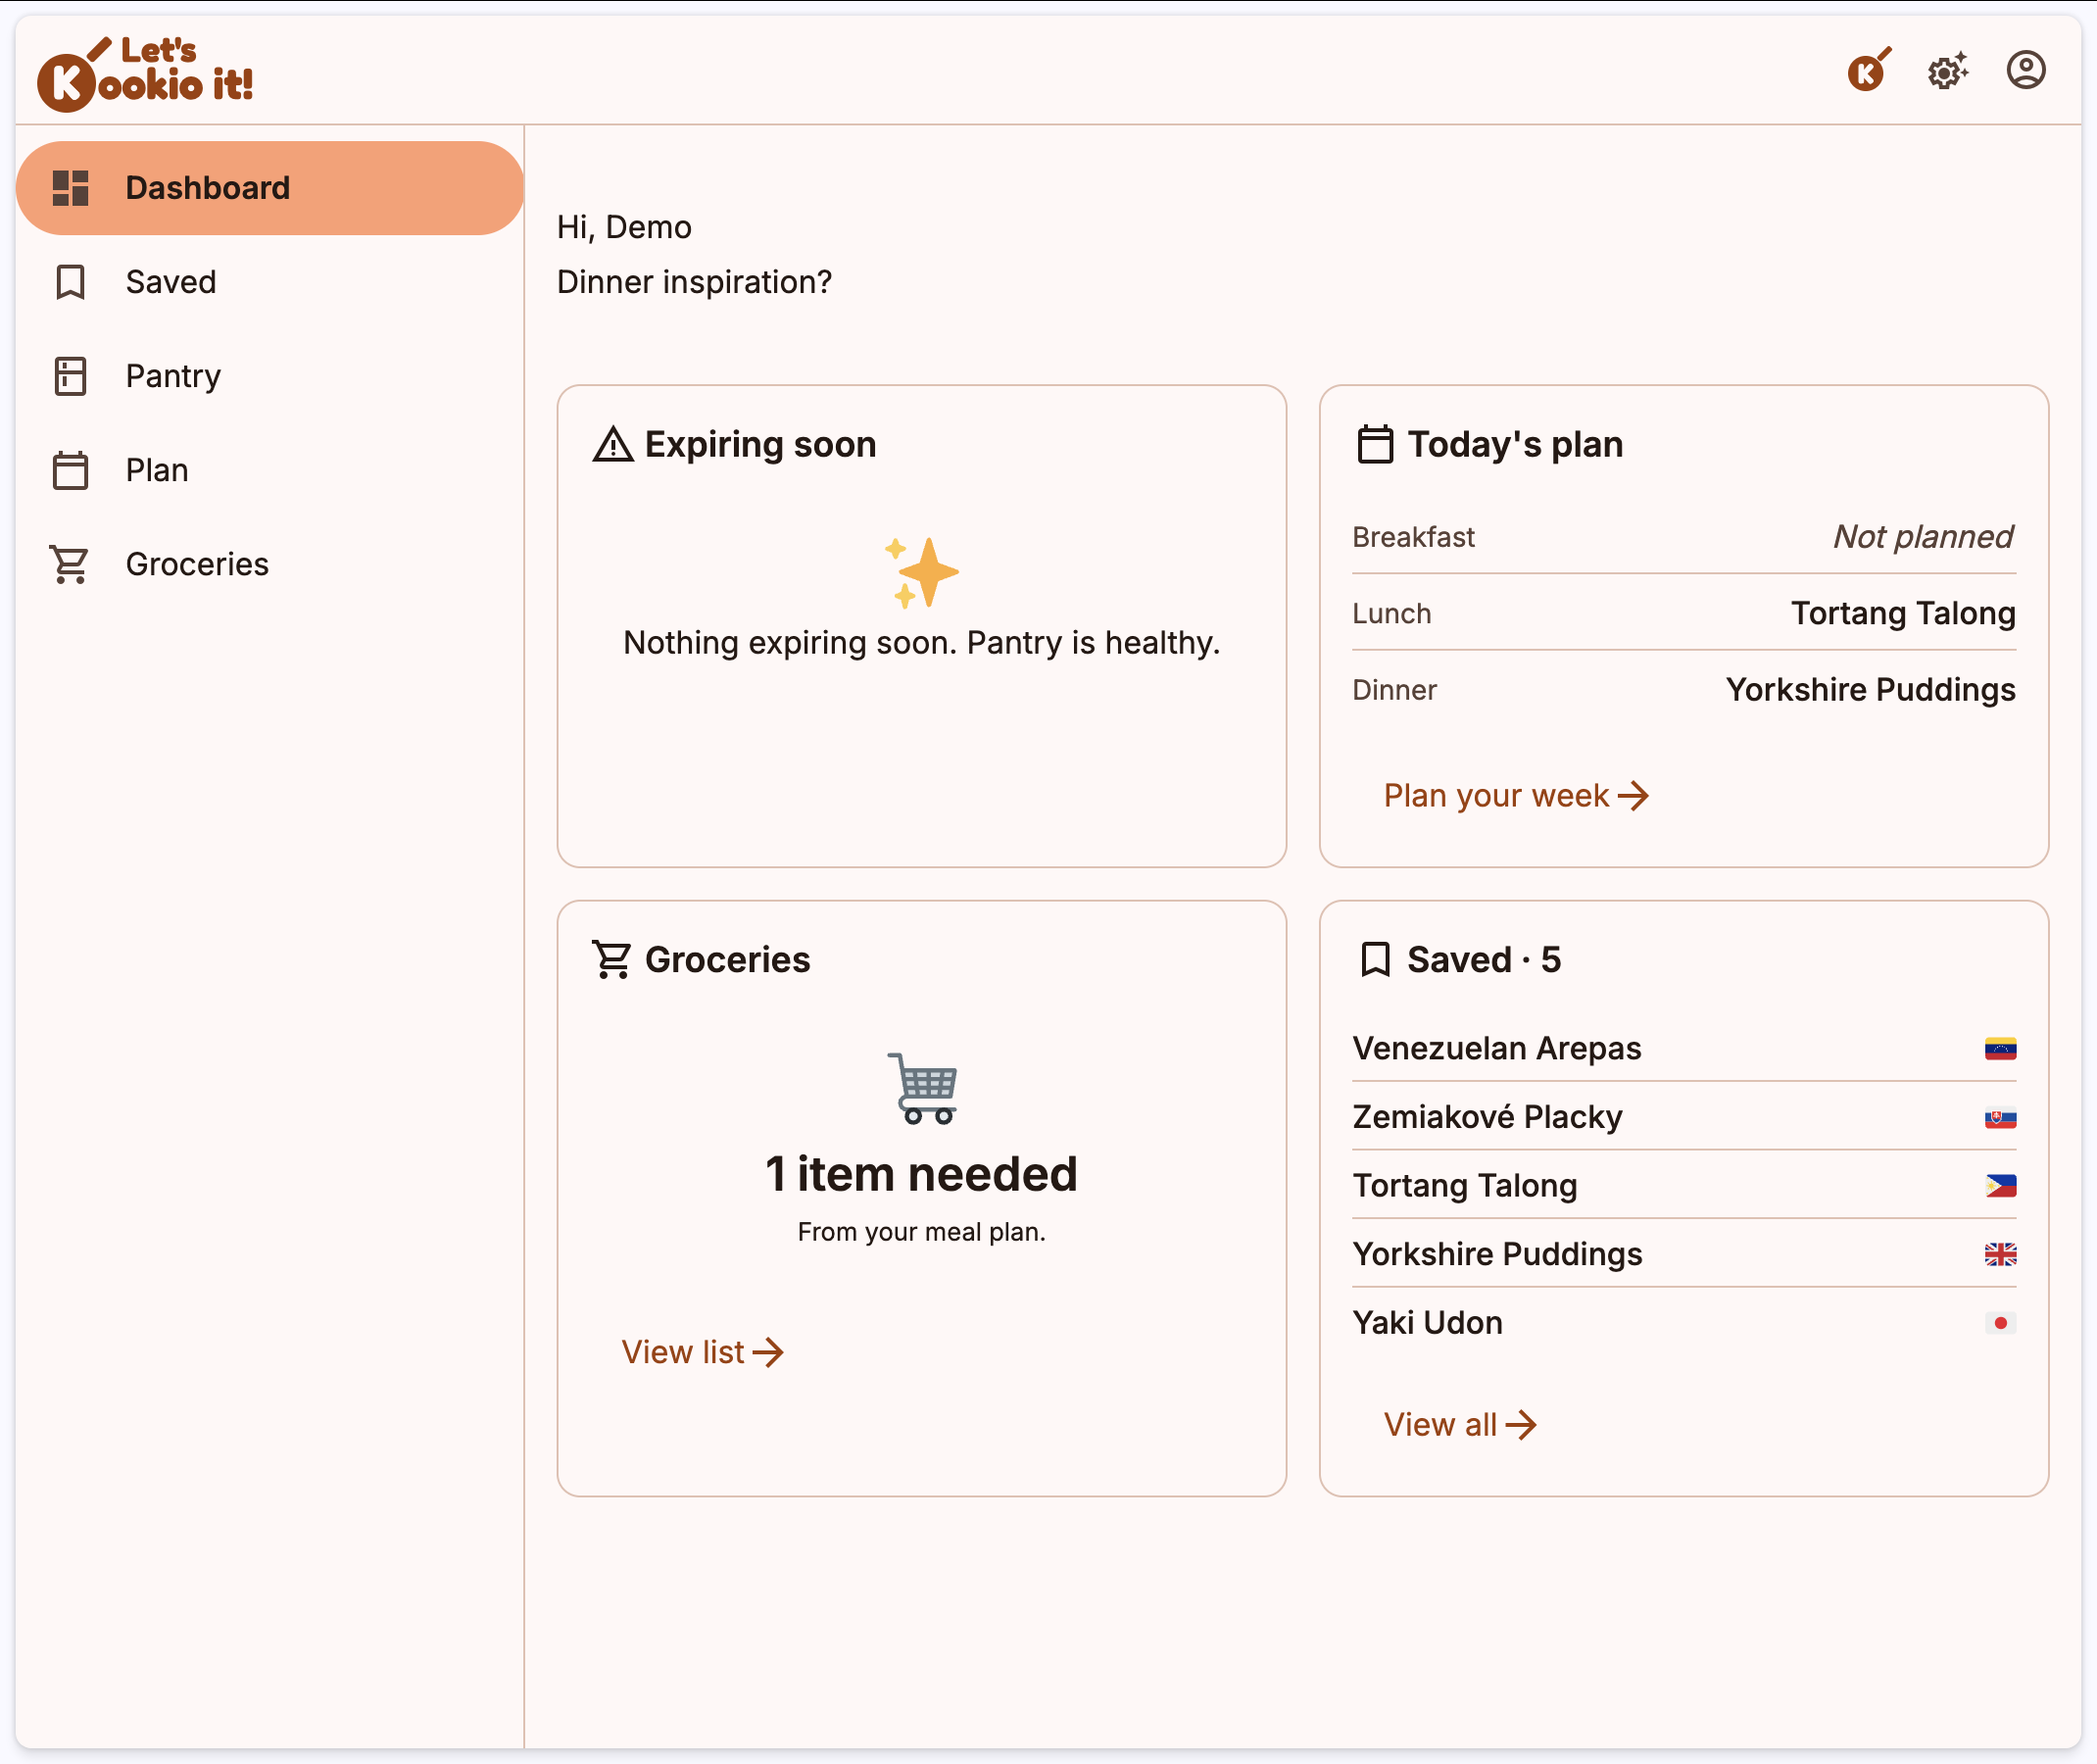
\includegraphics[width=0.66\textwidth]{kookio-demo-dashboard}
  \caption{The dashboard (\texttt{/dashboard}): the entry point after authentication, with access to the application's flows and a summary of the current state.}
  \label{fig:demo-dashboard}
\end{figure}

\begin{figure}[htbp]
  \centering
  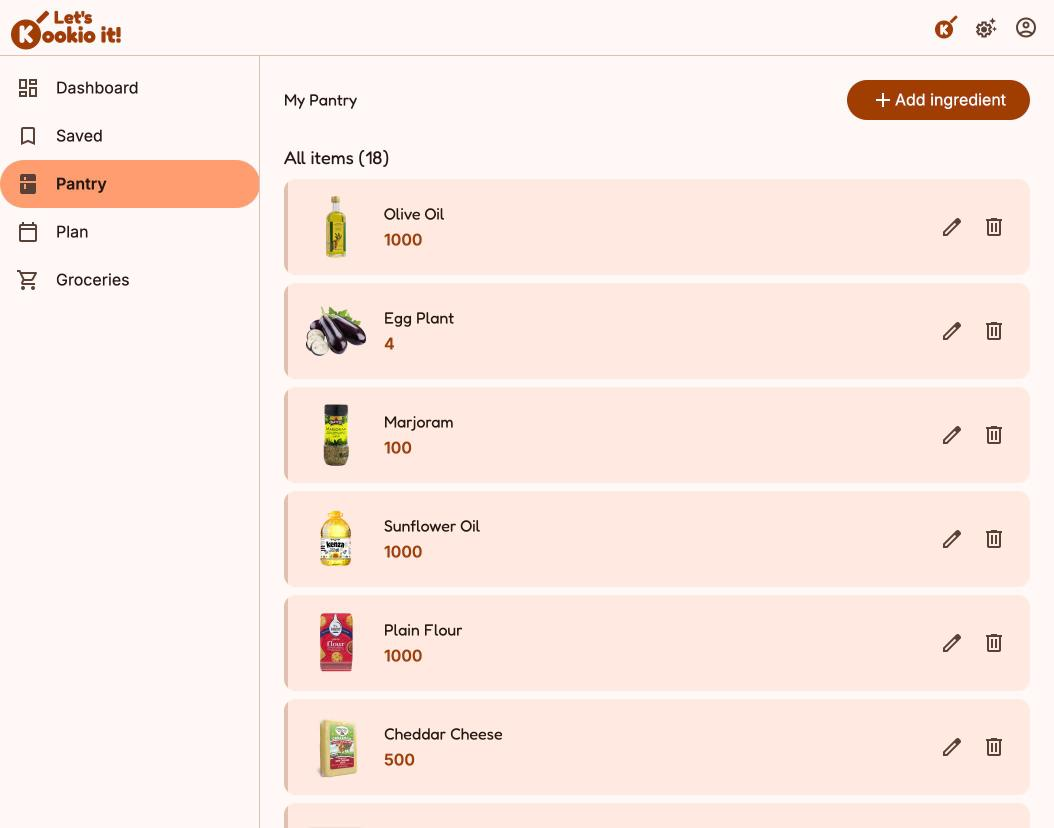
\includegraphics[width=0.66\textwidth]{kookio-demo-pantry}
  \caption{The pantry (\texttt{/pantry}): the user's inventory, with each ingredient stored in its display unit. This is the starting point of the flow --- the source of truth for what is available at home.}
  \label{fig:demo-pantry}
\end{figure}

\begin{figure}[htbp]
  \centering
  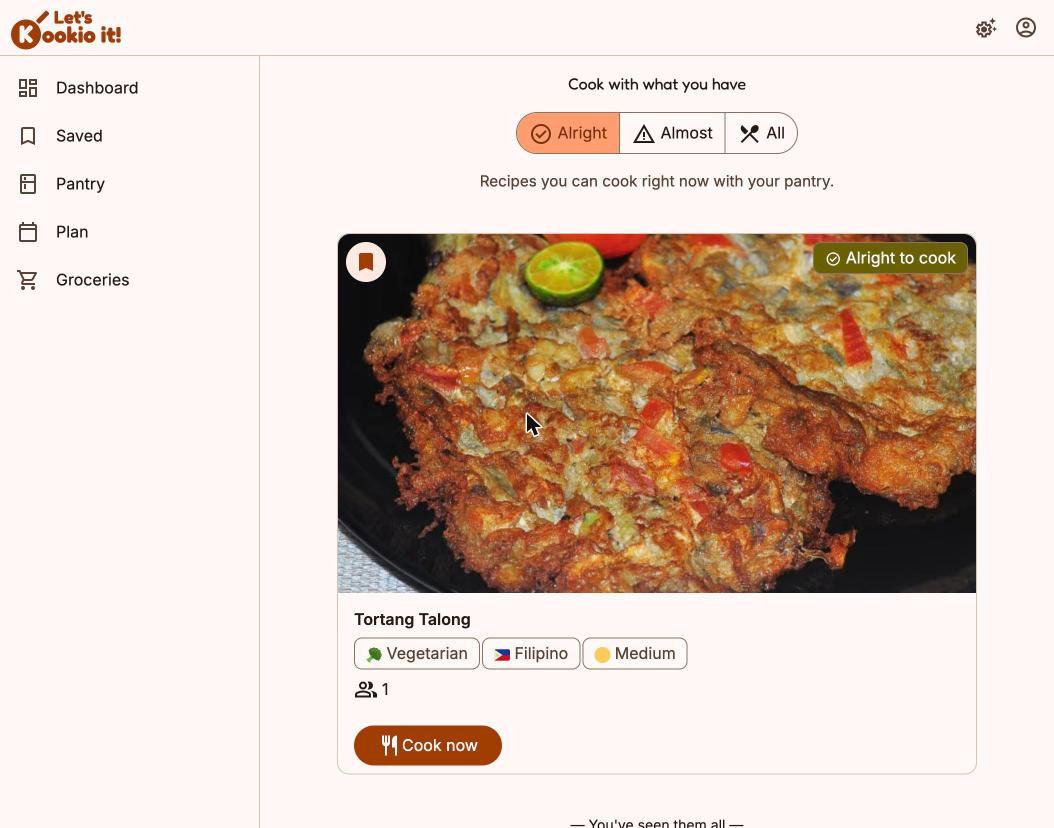
\includegraphics[width=0.66\textwidth]{kookio-demo-match}
  \caption{Progressive filtering (\texttt{/recipes/match}): the catalog partitioned by the degree of coverage from the pantry (\secref{subsec:filtru-progresiv}). The \textit{Alright} level lists the fully covered recipes, \textit{Almost} those missing one to three ingredients.}
  \label{fig:demo-match}
\end{figure}

\begin{figure}[htbp]
  \centering
  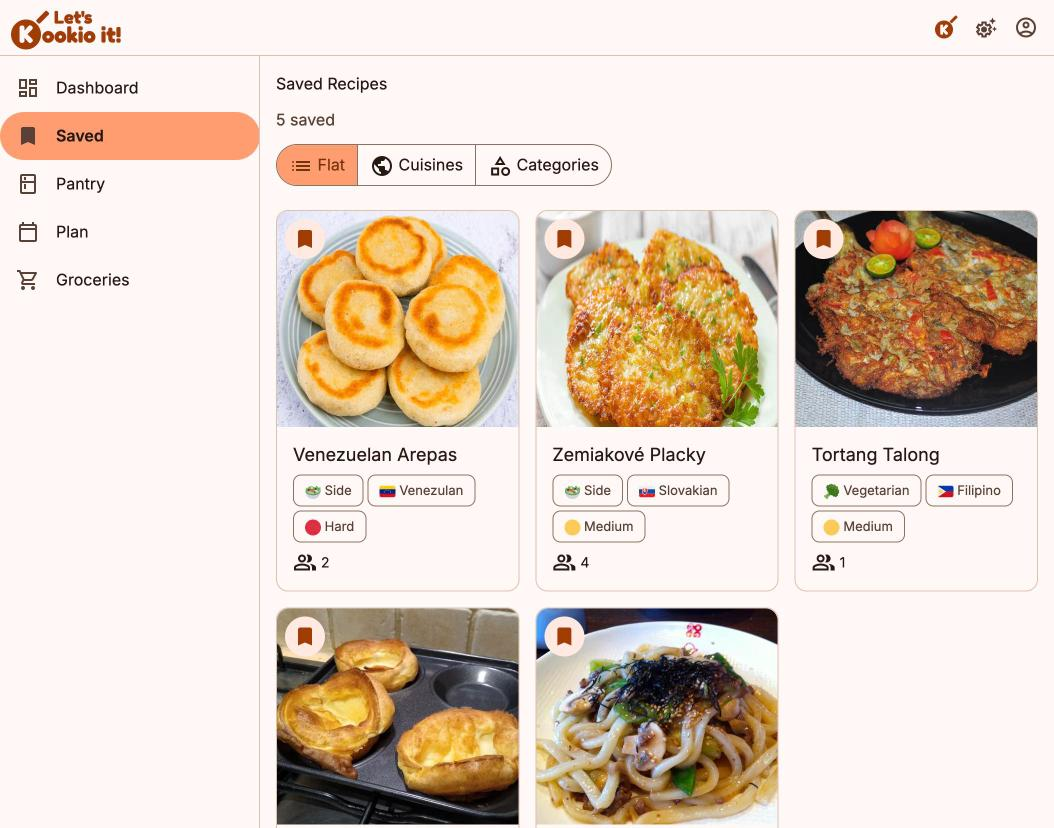
\includegraphics[width=0.66\textwidth]{kookio-demo-saved}
  \caption{Saved recipes (\texttt{/recipes/saved}): the collection of recipes marked by the user for later access, independent of the degree of coverage from the pantry.}
  \label{fig:demo-saved}
\end{figure}

\begin{figure}[htbp]
  \centering
  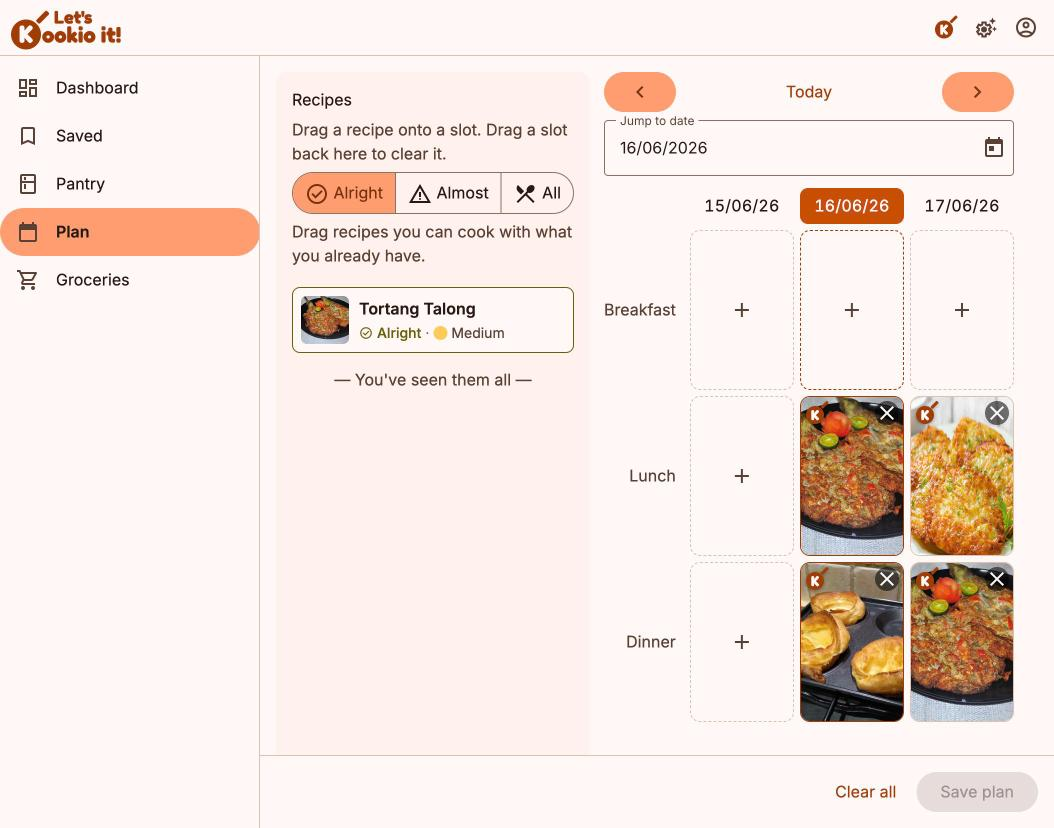
\includegraphics[width=0.66\textwidth]{kookio-demo-plan}
  \caption{The planner (\texttt{/plan}): recipes are assigned to \texttt{(date, meal type)} slots, modeled as \texttt{MealSlot} with the \texttt{@@unique} constraint described in \secref{subsec:gestionarea-datelor}.}
  \label{fig:demo-plan}
\end{figure}

\begin{figure}[htbp]
  \centering
  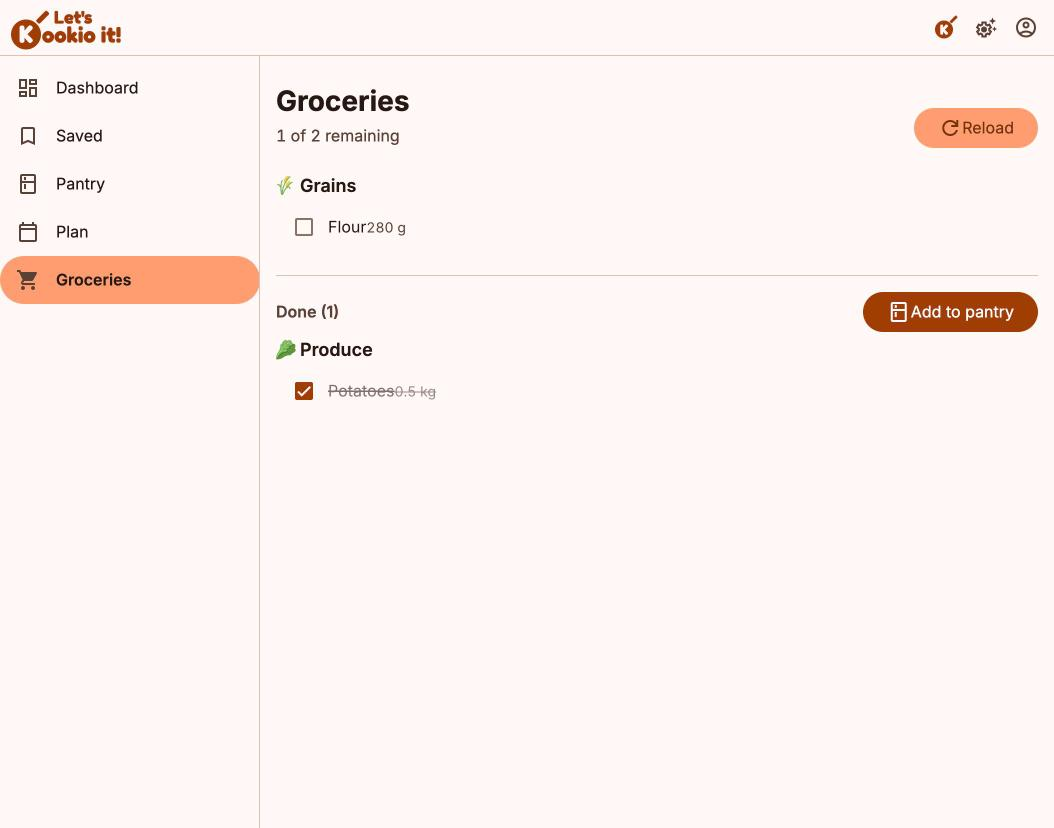
\includegraphics[width=0.66\textwidth]{kookio-demo-groceries}
  \caption{The shopping list (\texttt{/groceries}): the set difference between the ingredients of the planned slots and the contents of the pantry (\secref{subsec:lista-cumparaturi}). Items checked as “bought” can be merged back into the pantry.}
  \label{fig:demo-groceries}
\end{figure}

\begin{figure}[htbp]
  \centering
  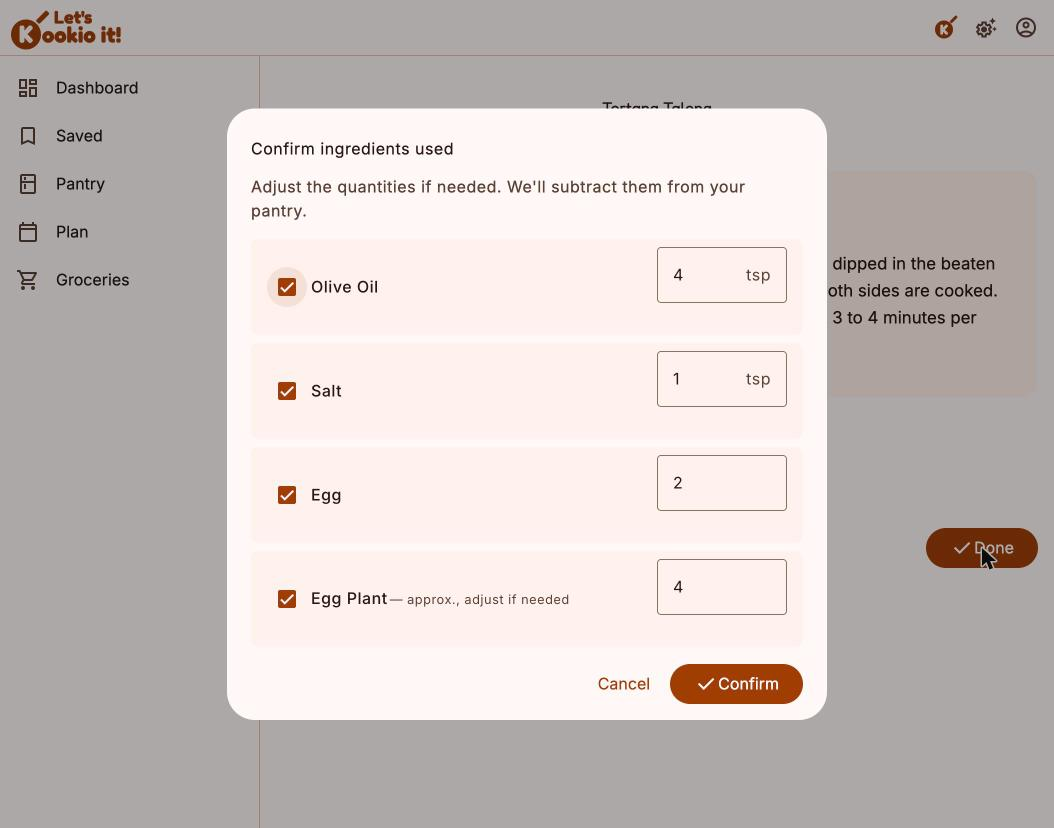
\includegraphics[width=0.66\textwidth]{kookio-demo-cook}
  \caption{The cooking session (\texttt{/cook/:recipeId}): at the end, the dialog offers the pre-filled consumed quantities, and the confirmation triggers the transactional decrementing of the pantry (\secref{subsec:sesiune-gatit}).}
  \label{fig:demo-cook}
\end{figure}

\subsection{Details of the unit conversion pipeline}\label{anexa:grams-detail}

The body of the thesis (\secref{subsec:algoritm-grame}) keeps the unit conversion pipeline at the level of the design decision --- the pair of pure functions \texttt{toGrams}/\texttt{fromGrams} as an application of information hiding. The concrete detail of the conversion rules is relocated here, being an implementation detail specific to the application, useful as a reference, but not necessary for the architectural argument.

The pipeline handles four classes of units, each with an explicit rule:

\begin{itemize}
  \item \textbf{Weight} (\texttt{G}, \texttt{KG}, \texttt{OZ}, \texttt{LB}): direct conversion through constant factors.
  \item \textbf{Volume} (\texttt{ML}, \texttt{L}, \texttt{TSP}, \texttt{TBSP}, \texttt{CUP}): conversion through the density of water (\texttt{1 ml} \(\approx\) \texttt{1 g}), an acceptable approximation for the ingredients commonly used in home cooking.
  \item \textbf{Pieces} (\texttt{PIECE}, \texttt{SLICE}, \texttt{CLOVE}, \texttt{BUNCH}, \texttt{OTHER}): conversion through the optional \texttt{IngredientCatalog.\allowbreak pieceGrams} column (\texttt{Float?}), populated with 32 values (\texttt{egg: 60}, \texttt{garlic clove: 5}, \texttt{lemon: 100} etc.).
  \item \textbf{Taste and garnish} (\texttt{TO\_TASTE}, \texttt{TO\_SERVE}, \texttt{GARNISH}): treated as \texttt{0 g} and excluded from the shopping list. The distinction from \texttt{PINCH} is not one of size, but of nature: \texttt{PINCH} is a quantity specified by the recipe's author (a pinch), whereas the taste and garnish units express an instruction --- “to taste”, “to serve” --- whose quantity is deliberately left to the discretion of whoever is cooking. The \texttt{0 g} value is therefore a consciously chosen modeling convention, not an unknown: it honors the author's intention (assigning a gram-equivalent would override a decision explicitly left open), avoids downstream noise (half a gram of salt decremented on every cooking session, or staple seasonings listed for shopping, are not useful information in an application focused on the waste of bulk food) and keeps a neutral position with respect to dietary intake, which the application is not in a position to prescribe. For \texttt{PINCH}, on the other hand, a convention sets \texttt{0.5 g} per unit --- a small but real mass, enough to allow sub-pinch rows to be deleted from the pantry.
\end{itemize}

For piece-type ingredients without a populated \texttt{pieceGrams} value, the function returns \texttt{null}, signaling to the caller that it cannot produce an estimate. An optional \texttt{allowDefault} parameter changes this behavior: when explicitly enabled, the function returns \texttt{DEFAULT\_PIECE\_GRAMS = 100} g per piece. The \(100\) g value is a rough approximation, chosen as a plausible order of magnitude for an arbitrary piece, not an empirically measured average; its role is that of a safety net, not of an exact estimate --- which is why it is not applied by default, but only at the caller's explicit request. This option protects the callers that prefer an explicit error (the cooking session, where an unfounded consumption would corrupt the inventory) from silently accepting unreliable estimates, while allowing the consumers that prefer graceful degradation (the shopping list, where an approximate estimate is preferable to a total failure) to continue processing.

\lstref{lst:to-grams} presents the \texttt{toGrams} function. The complete implementation, together with the inverse \texttt{fromGrams}, is located in \texttt{libs/\allowbreak shared/\allowbreak utility/\allowbreak src/\allowbreak lib/\allowbreak labeling/\allowbreak measure-unit-labels.ts}.

% Code listing — manual numbering via the codlista float counter
% (\refstepcounter{codlista} + minipage + Verbatim from fancyvrb), keeping a
% single listing style across the document.
\refstepcounter{codlista}\label{lst:to-grams}
\par\medskip
\noindent\begin{minipage}{\linewidth}
\textbf{Listing \thecodlista:} The \texttt{toGrams} function --- normalizing quantities to grams.
\begin{Verbatim}[fontsize=\small]
export const toGrams = (
  amount: number,
  unit: MeasureUnit,
  pieceGrams: number | null = null,
  opts: GramsConversionOptions = {},
): number | null => {
  if (FLAVOUR_ONLY_UNITS.has(unit)) return 0;

  const fixed = UNIT_TO_GRAMS_FIXED[unit];
  if (fixed !== undefined) return amount * fixed;

  // Piece-class: PIECE, SLICE, CLOVE, BUNCH, OTHER.
  const piece =
    pieceGrams !== null && pieceGrams > 0
      ? pieceGrams
      : opts.allowDefault
        ? DEFAULT_PIECE_GRAMS
        : null;
  if (piece === null) return null;
  return amount * piece;
};
\end{Verbatim}
\end{minipage}
\par\medskip
% 5-appendix-demo.tex ends here

\clearpage
% 5-appendix-c.tex starts here
% \raggedbottom for the appendix: the intro paragraph shares a page with no
% float (the ER diagram is [p], on its own page), so \flushbottom from the body
% would stretch that short paragraph's vertical glue into big gaps. Previously
% set by the now-removed LaTeX-tooling and PAN-manifest appendices.
\raggedbottom

\section{The data model}\label{anexa:model-date}

The complete database schema --- the 20 \gls{prisma} models --- is shown in
\figref{fig:er-diagram} as an entity-relationship diagram. The diagram is
generated automatically from \texttt{schema.prisma} (with
\textit{prisma-dbml-generator}) and rendered with \textit{dbdocs.io}, so it
stays in sync with the actual data model. Primary keys are marked with the key
symbol, foreign keys with the link symbol, and the connectors between tables
show the relationships between entities; the junction tables (for example
\texttt{UserDietaryRestriction}, \texttt{RecipeCollectionEntry}) are placed next
to the entities they link.

\begin{figure}[p]
  \centering
  % Image is the dbdocs PDF export cropped to its content with `pdfcrop` ---
  % the raw export carries a full-canvas white border that wastes ~1/3 of the
  % page. Re-crop after any re-export. keepaspectratio + the height cap keep
  % the diagram inside the text block.
  \makebox[\textwidth]{%
    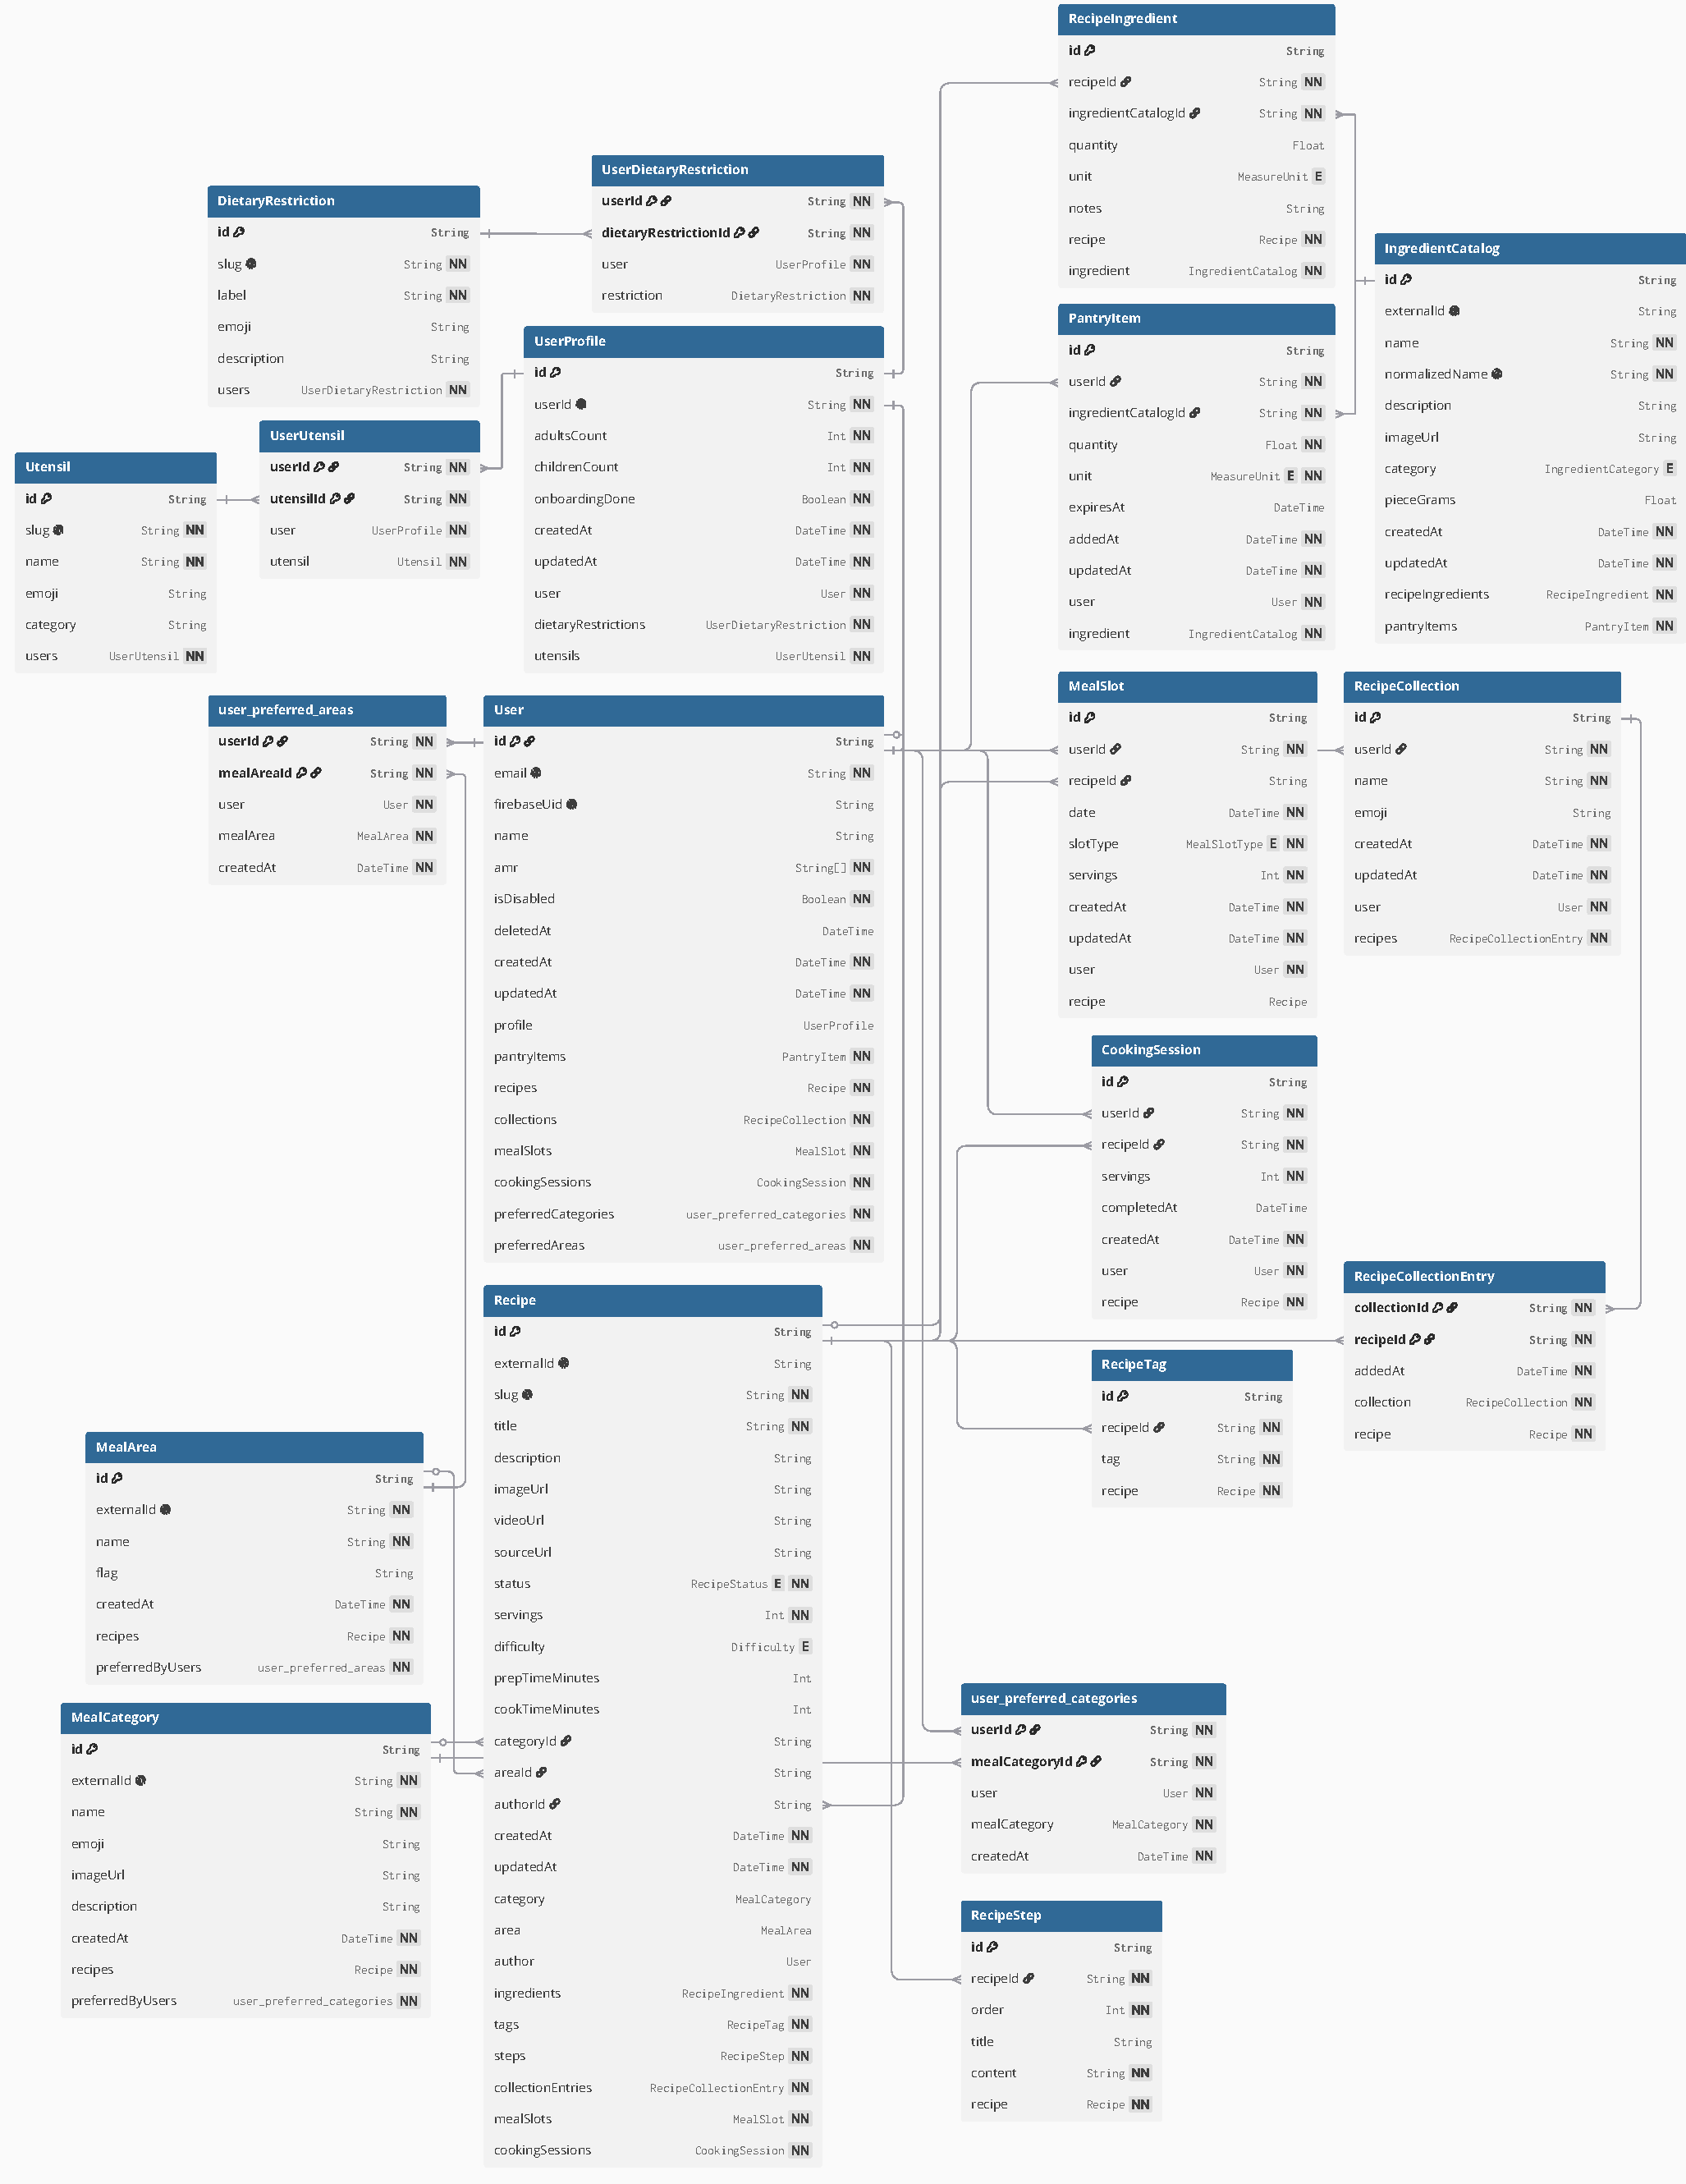
\includegraphics[width=\textwidth,height=0.9\textheight,keepaspectratio]{kookio-er-diagram}}
  \caption[Entity-relationship diagram of the database]{Entity-relationship
    diagram of the data schema: the 20 models and the relationships between
    them, generated from \texttt{schema.prisma} and published on
    \textit{dbdocs.io}. The interactive, browsable version:
    \url{https://dbdocs.io/dinea.eduard/kookio-db} (access password:
    \texttt{FMI\_2026}).}
  \label{fig:er-diagram}
\end{figure}

% 5-appendix-c.tex ends here

\clearpage
\end{appendices}

% Glossary and bibliography stay single-spaced with ragged bottom — same
% rationale as TOC (reference apparatus, not body text). The `\raggedbottom`
% prevents last-line clipping; entries land cleanly before page boundary.
\raggedbottom
\begingroup
\singlespacing
\setlength{\parskip}{0pt}
\glsaddall
\printglossary[title={Glossary of Terms}]
\clearpage
\printglossary[type=\acronymtype,title={List of Acronyms}]
\clearpage
\printbibliography
\endgroup
\end{document}
% main.tex ends here